\documentclass[a4paper,landscape]{article}
\usepackage{fontspec}
\newfontfamily{\demo}{TeX Gyre Pagella}
\DeclareTextFontCommand{\textdemo}{\demo}
\usepackage{unicode-math}
\usepackage[inner=1in,textwidth=5in,textheight=6in, marginparsep=0.5in, marginparwidth=4.2in]{geometry}
\usepackage{sectsty}
\allsectionsfont{\normalfont\sffamily\bfseries}
\usepackage{fancyvrb}\fvset{fontsize=\small}
\usepackage{xcolor}
\usepackage{graphicx}
\usepackage{mflogo}
\def\mfbook{\textsl{The \MF\kern1pt book}}
\def\texbook{\textsl{The \TeX\kern1pt book}}
\usepackage{shortvrb}\MakeShortVerb{"}
\usepackage{listings}
\title{Drawing with Metapost}
\author{Toby Thurston}
\date{March 2017}
\overfullrule=2pt
\def\kw#1{\begingroup\def\_{\kern.04em
    \vbox{\hrule width.3em height .6pt}\kern.08em}%
\ifmmode\mathop{\textbf{#1}}\else\hbox{\bf#1\/}\fi\endgroup}
\def\op#1{\begingroup\def\_{\kern.04em
    \vbox{\hrule width.3em height .6pt}\kern.08em}%
\ifmmode\mathop{\textrm{#1}}\else\hbox{\rm#1\/}\fi/color\endgroup}
\def\id#1{\begingroup\def\_{\kern.04em
    \vbox{\hrule width.3em height .6pt}\kern.08em}%
\ifmmode\mathop{\textit{#1}}\else\hbox{\it#1\/}\fi\endgroup}
\def\cycle{{\rm cycle}}
\def\vpic#1#2{\moveright5.5in\vbox to 0pt{\vskip#1\includegraphics{#2}\vss}}
\def\mpic#1#2{\vadjust{\moveright5.5in\vbox to 0pt{\hsize4in\vskip#1\centerline{\includegraphics{#2}}\vss}}}
\def\mwpic#1#2{\vadjust{\moveright5.5in\vbox to 0pt{\hsize4in\vskip#1\centerline{\includegraphics[width=4in]{#2}}\vss}}}
\def\nb{$\vcenter{\hbox{
\includegraphics[height=6pt]{ding1}}}$\ }
\def\unit#1{\ifmmode\,\else\thinspace\fi\hbox{#1}}
\def\to{\mathrel{\ldotp\ldotp}}
%
\definecolor{textblue}{rgb}{.2,.2,.7}
\definecolor{textred}{rgb}{0.54,0,0}
\definecolor{textgreen}{rgb}{0,0.43,0}
% style for highlighting
\newcommand\mpstyle{\lstset{
language=Metapost,
basicstyle=\ttfamily,
keywordstyle=\color{textblue},
commentstyle=\color{textred},    % Custom highlighting style
stringstyle=\color{textgreen},
frame=none,                      % Any extra options here
columns=fullflexible,
keepspaces=true,
xleftmargin=\parindent,
showstringspaces=false           % 
}}
\lstnewenvironment{smallcode}[1][]{\mpstyle\lstset{basicstyle=\small\ttfamily}}{}
\lstnewenvironment{code}[1][]{\mpstyle\lstset{#1}}{}
\newcommand\mpexternal[2][]{{\mpstyle\lstinputlisting[#1]{#2}}}
\newcommand\mpl[1]{{\mpstyle\lstinline!#1!}}
\begin{document}
\pagestyle{empty}
\raggedbottom
% title & toc in the margin
\makeatletter
\moveright 6in\vbox to
0pt{\vskip23pt\noindent\sffamily{\Large\bfseries\@title}\par\bigskip
    \noindent\@author\ --- \@date\par
    \bigskip
    \halign{\hfil#\hfil\ &\hfil#\hfil\cr
    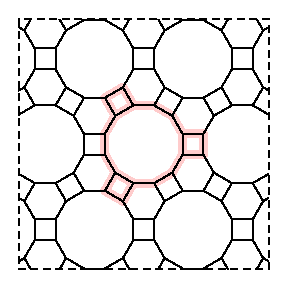
\includegraphics{archimedes1}&
    
\includegraphics{archimedes2}\cr
    $(4,6,12)$ & $(4,8^2)$\cr
    \noalign{\medskip}
    
\includegraphics{archimedes3}&
    
\includegraphics{archimedes5}\cr
$(3,12^2)$ & $(3,4,6,4)$\cr}
\vss}
\makeatother
\section{Start here}

This document contains a collection of ideas and techniques for producing attractive
technical drawings with John Hobby’s \MP\ language.  I’m assuming that you already
know the basics of the language, that you have it installed as part of your up to
date \TeX\ ecosystem, and that you have established a reasonable work-flow that
let’s you write a Metapost program, compile it, and include the results in your
\TeX\ document.  If not, you might like to start at the \MP\ page on CTAN, and read
some of the excellent tutorials, including "mpintro.pdf".  If you have already done
this, please read on.

These notes are based on the many examples I have developed as answers
to questions about technical drawing on the wonderful \TeX\ StackExchange site.  In
accordance with their terms and conditions, I’ve only included material here that
I’ve written myself --- if you want other people’s code then visit the site;
while most answers there focus on writing \LaTeX\ documents, there are a great
many questions about drawing, and some of the answers are very illuminating.  

My approach here will be to explore plain \MP, with examples grouped
into themes.  One approach to using this document would be to read it end to end.
Another would be to flick through until you see something that looks like it might
be useful and then see how it’s done. 

And when I say \textit{plain} \MP\ I mean \MP\ with the default format (as defined
in the file "plain.mp") loaded and no other external packages (apart from "boxes.mp"
very occasionally).  Nearly all of the examples here are supposed to be self
contained, and any macros are defined locally so you can get to grips with what’s
going on.  \MP\ is a very subtle language, and it’s possible to do some
very clever and completely inscrutable things with it;  in contrast I’ve tried to be
as clear as possible in my examples.

\newpage
\section{Some features of the syntax}

\begin{itemize}
    \item Assignment or equation:  the equation "a=3;" means "a" is the same as "3" throughout the
        current scope; the assignment "a:=3;" means update the value of "a" to the value "3"
        immediately.  The difference becomes apparent when you try to update a
        variable in the same scope.  
        \mwpic{0pt}{tiling}
        
        This difference also lets you write linear equations
        like "a=-b;".  After this, as soon as you give  a value to "a", \MP\ immediately works
        out the value of "b".  
        This is clever but has its limitations.  As the following snippet reveals:
\begin{code}
  % if you run this       you will get this in the log
  a + b = 0; show (a,b);  % >> (a,-a)
  a=42;      show (a,b);  % >> (42,-42)
  a:=43;     show (a,b);  % >> (43,-42)
\end{code}
        As soon as you assign to variable with ":=" \MP\ breaks any previously
        established equations.

    \item Variable types: 
        
        —
        \mpl{numeric} "a", 
        \mpl{pair} "(a,b)"

        —
        \mpl{color} "(r,g,b)",
        \mpl{color} "(c,m,y,k)"
        \mpl{transform} "(x,y,xx,xy,yx,yy)"

        —
        \mpl{string},
        \mpl{path},
        \mpl{picture}


        If you don’t declare a variable, it’s assumed that it’s a \mpl{numeric}.
        When you do declare a variable --- \mpl{numeric} or otherwise — any value that it
       already had in the current scope is removed.
            
    \item Implicit multiplication: \MP\ inherits a rich set of rules about numerical
        expressions from \MF, and of special interest is the scalar multiplication
        operator.  Any simple number, like "42", "3.1415", or ".6931", or any simple
        fraction like "1/2" or "355/113" standing on it’s own (technically at the
        primary level) and not followed by "+" or "-" becomes a scalar
        multiplication operator that applies to the next token (which should be variable 
        of some appropriate type).
        So you can write things like "3a", or even "1/2 a"
        (the space between the number and the variable name is optional). This 
        lets you write very readable mathematical expressions. It’s quite
        additictive after a while.


\end{itemize}
    
    

\newpage
\section{Making and using closed paths}
\label{plain-shapes}

In \MP\ there are two sorts of paths: open and closed.  
\mpic{-12pt}{closed0}
A closed path is called a cycle, and is created with the "cycle" primitive like this:
\begin{code}
path t; t = origin -- (55,0) -- (55,34) -- cycle;
\end{code}
You can think of "cycle" as meaning ‘connect back to the start and close the path’.
You can use "draw" with either sort of path, but you can only use "fill" with a
cycle.  This concept is common to most drawing languages but it’s often hidden:  an
open path might be automatically closed for you when you try to fill it.  \MP\ takes
a more cautious approach; if you pass an open path to "fill" you will get an error
that says ‘Not a cycle’.  You can also use "cycle" in a boolean context to test
whether a path "p" is cyclic: 
$\hbox{\ttfamily if cycle p: ... fi}$.

\medskip\noindent
There are several closed paths defined for you in plain \MP. 
\mpic{1cm}{closed7}
\begin{itemize}
    \item "unitsquare" which you can use to draw any rectangle with appropriate
        use of "xscaled" and "yscaled" --- it’s defined so that the bottom left
        corner is point 0 of the shape.  This point is also defined as "(0,0)", 
        so the "unitsquare" is centred on point "(1/2,1/2)".  If you want a square
        centered on the origin, then shift it by "-(1/2,1/2)" before you scale it.

    \item "fullcircle" which you can use to draw any circle or ellipse with
        appropriate use of "xscaled" and "yscaled".  Defined so that it is centered
        at the origin and has unit \textit{diameter} and point 0 is "(1/2,0)".

    \item "superellipse()" which creates the shape beloved of the Danish designer Piet Hein.  Unlike the
        other two, this one is a function rather than a path, so you need to call it
        like this:
        \begin{code}
        path s; s = superellipse(right,up,left,down,.8);
\end{code}
        to create a ‘unit’ shape.  The fifth parameter is the ‘superness’: the value
        1 makes it look almost square, 0.8 is about right, 0.5 gives you a diamond,
        and values outside the range $(0.5,1)$ give you rather weird propeller
        shapes.
\end{itemize}

\newpage\subsection{Points on the standard closed paths}\noindent\mpic{-10pt}{closed1}%
Here are the three shapes centered on the origin and labelled to show the points
along them.  \textbf{Note} that the \textit{unitsquare} shape has been shifted so that it is
centered on the origin in all of these examples.  The small red circle marks the
\textit{origin}, and the labelled red dots are the points of each path.  The
\textit{unitsquare} has four points, while the other two shapes both have eight.
The small
arrows between point~0 and point~1 of each shape indicate the direction of the path
that makes up the shape.  

\vfill\noindent
If you want to highlight a segment of your shape, there’s a neat way to define it
using "subpath".  Assuming "p" is the path of your shape, then this:
\begin{code}
center p -- subpath(1,2) of p -- cycle
\end{code}
creates a useful wedge shape which looks like this in our three ‘standard’
shapes.

\vfill\noindent
Better still, you are not limited to integer points along the path of your closed shape.
So if you wanted a wedge that was exactly $1/5$ of the area of your shape, you
could try
\begin{code}
center p -- subpath(0,1/5 length p) of p -- cycle
\end{code}

Clearly this works rather better with more circular shapes.  Indeed for a circle you
can convert directly between circumference angle and points along the path.  So
you have defined path "c" to be a circle, then
"point 1 of c" is $45^\circ$ round and 1~radian is "point 1.27324 of c", (because
$4/\pi \simeq 1.27324$).

\vfill\noindent
In a cyclic path, the point numbering in \MP\ wraps round: so in a
circle, point $n$ is the same as point $n+8$; and in general point $n$ is the same as
point $n+\hbox{\bf length }p$.  This works with negative numbers too, so we could use 
\begin{code}
center p -- subpath(-1,1) of p -- cycle
\end{code}
to get wedge centered on point 0.

\newpage\subsection{Building cycles from parts of other paths}

Plain \MP\ has a built-in function to compute the intersection points of two paths, and
there’s a handy high level function called "buildcycle" that uses this function to
create an arbitrary closed path.  
\mpic{0pt}{area-under-graph1}
The arguments to the function are just a list of paths, and providing the paths all
intersect sensibly, it
returns a cyclic path that can be filled or drawn.  This is often used for colouring an
area under a function in a graph.
Here is an example. The red line has been defined
as path "f" and the two axes as paths "xx", and "yy".  The blue area was defined
with
\begin{code}
buildcycle(yy shifted (1u,0), f, yy shifted (2.71828u,0), xx)
\end{code}
Note the use of the $y$-axis shifted along by different amounts.

\smallskip\noindent
There are similar examples in the \MP\ manual, but "buildcycle" can also
be useful in more creative graphics.
Here’s a second example that uses closed paths to give an illlusion of depth to a simple
graphic of the planet Saturn.
\mpic{0pt}{saturn1}
\marginpar{\hbox{}\vskip1.3in\raggedright\noindent\textbf{Notes}\begin{itemize}
    \item The first five paths are just circles and ellipses based on "fullcircle".
    \item The drawing is done inside an "image" simply so that the final result can
        be drawn at an angle
    \item "unfill gap" is shorthand for "fill gap withcolor background"
    \item The subpaths passed to "buildcycle" are chosen carefully to make sure we
        get the intersections at the right points and so that the component paths
        all run in the same direction.  Note that "subpath (8,4) of globe" runs
        clockwise (that is backwards) from point 8 to point 4.
\end{itemize}}
\mpexternal{saturn.mp}

\newpage\subsection{The implementation of \texttt{buildcycle}}
\textsc{The implementation} of "buildcycle" in plain \MP\ is interesting for a number of
reasons.  Here it is copied from "plain.mp" (with minor simplifications) $\longrightarrow$
\vadjust{\moveright5.5in\vbox to 0pt{\kern-1cm%
\begin{code}
vardef buildcycle(text input_path_list) =
  save ta, tb, k, j, pp; path pp[];
  k=0;
  for p=input_path_list: pp[incr k]=p; endfor
  j=k;
  for i=1 upto k:
    (ta[i], length pp[j]-tb[j]) 
      = pp[i] intersectiontimes reverse pp[j];
    if ta[i]<0:
      errmessage("Paths " & decimal i &
                  " and " & decimal j & " don't intersect");
    fi
    j := i;
  endfor
  for i=1 upto k: 
    subpath (ta[i],tb[i]) of pp[i] .. 
  endfor cycle
enddef;
\end{code}
\vss}}

\noindent
Notice how freely the indentation can vary; this is both a blessing 
(because you can line up things clearly) and a curse (because the syntax may not
be very obvious at first glance).  Notice also the different ways we can use a
$\kw{for}$-loop.  The first two are used at the ‘outer’ level to repeat complete
statements (that end with semi-colons); the third one is used at the ‘inner’ level
to build up a single statement.

The use of a "text" parameter allows us to pass a comma-separated list as an
argument; in this case the list is supposed to be a list of path expressions that
(we hope) will make up a cycle.  The first "for" loop provides us with a standard
idiom to split a list; in this case the comma-separated value of "input_path_list"
is separated into into a more convenient array of paths called "pp" indexed by "k".
Note that the declaration of the array as "path" forces the argument to be a list of
paths.

The second "for" loop steps through this array of paths looking for intersections.
The index "j" is set to be "k" when "i=1", and then set to the previous value of "i"
at the end of the loop;   in this way
"pp[j]" is the path before "pp[i]" in what is supposed to be a cycle.
The macro uses the primitive operator \mpl{intersectiontimes} to find the intersection
points, if any. Note that we are looking for two path times: the time to start a
subpath of the current path and the time to end a subpath of the previous path; the
macro does this neatly 
by reversing the previous path and setting the $b$-point indirectly by subtracting
the time returned from the length of the path. 

If all has gone well, then "ta" will hold all the start points of the desired
subpaths, and "tb" all the corresponding end
points.
The third and final "for" loop assumes that this is indeed the case, and tries to 
connect them all together.  Note that it uses ".." rather than "&" just in case the
points are not quite co-incident; finally it finishes with a
"cycle" to close the path even though point "tb" of path "k" should be identical (or
at least very close) to 
point "ta" of path "0".

This implementation of \mpl{buildcycle} works well in most cases, provided that there
are enough components to the cycle of paths.  If you only have two paths, then the
two paths need to be running the same direction, and the start of each path must not
be contains within the other.  This is explored in the next section.

\newpage
\subsection{Strange behaviour of \texttt{buildcycle} with two cyclic paths}

The implementation of "buildcycle" in plain \MP\ can get confused if you use it with
just two paths.  Consider the following example: \mpic{0pt}{overlaps2}
\begin{code}
beginfig(1);
  path A, B;  
  A = fullcircle scaled 2.5cm; 
  B = fullcircle scaled 1.8cm shifted (1cm,0);
  fill buildcycle(A,B) withcolor .8[blue,white]; 
  drawarrow A; drawarrow B;
endfig;
\end{code}
When we compile this example, we get no error message from "buildcycle", but there 
is no fill colour visible in the output.  The problem is that the points found by
"buildcycle" are the same both times that it steps through the middle loop, so
the cyclic path it returns consists of two identical (or very close) points and the 
so the fill has zero area.  

Now observe what happens when we rotate and reverse each of the paths in
turn.\mpic{-24pt}{overlaps3}
Number 1 corresponds to the example shown above; point~0 of~$A$ is inside the closed
path $B$.  In~2 we have rotated path $A$ by 180° so that the start of path~$A$ is no
longer inside $B$, and now "buildcycle" works ‘properly’ --- but this is the only
time it does so.  In~3, we've rotated $B$ by 180° as well, so that $B$ starts inside
$A$ and as expected "buildcycle" fails.  In 4 we've rotated $A$ back to it's
original position, so that both paths start inside each other; and we get the
union of the two shapes.  In 5--8, we've repeated the exercise with path $A$
reversed, and "buildcycle" fails in yet more interesting ways.  

You could use this behaviour as a feature if you need to treat $A$ and $B$ as sets
and you wanted to fill the intersection, union, or set differences, but if you just
wanted the overlap, then you need to ensure that both paths are running in the same
direction and that neither of them starts inside the other.
\marginpar{\small \nb To rotate a circular path, use: \texttt{p rotatedabout(center p,
180)}}

\newpage
\subsection{Find the overlap of two cyclic paths}

As we have seen, in order to get the overlap of two cyclic paths from "buildcycle",
we need both paths to be running in the same direction, and neither path should
start inside the other one.  It's not hard to create an "overlap" macro that does
this automatically for us.  The first element we need is a macro to determine if a
given point is inside a given closed path.  Following Robert Sedgwick's
\textit{Algorithms in C} we can write a generic "inside" function that works with any
simple closed path.  The approach is to extend a horizontal ray from
the point towards the right margin and to count how many times it crosses the cyclic
path; if the number is odd, the point must be inside.\vadjust{\moveright5.5in\vbox
    to 0pt{\kern-4.05cm
\begin{code}
vardef inside(expr p, ring) = 
  save t, count, test_line;
  count := 0;
  path test_line;
  test_line = p -- (infinity, ypart p);
  for i = 1 upto length ring:
     t := xpart(subpath(i-1,i) of ring 
                  intersectiontimes test_line);
     if ((0<=t) and (t<1)): count := count + 1; fi
  endfor
  odd(count)
enddef;
\end{code}
\vss}}\label{function:inside}

Equipped with this function we can create an "overlap" function that first uses the
handy "counterclockwise" function to ensure the given paths are running in the
same direction, and then uses "inside" to determine where the start points are.
\begin{smallcode}
vardef front_half primary p = subpath(0, 1/2 length p) of p enddef;
vardef back_half primary p = subpath(1/2 length p, length p) of p enddef;
% a and b should be cyclic paths...
vardef overlap(expr a, b) = 
  save A, B, p, q;
  path A, B; boolean p, q;
  A = counterclockwise a;
  B = counterclockwise b;
  p = not inside(point 0 of A, B);
  q = not inside(point 0 of B, A);
  if (p and q): 
    buildcycle(A,B)
  elseif p: 
    buildcycle(front_half B, A, back_half B)
  elseif q: 
    buildcycle(front_half A, B, back_half A)
  else: 
    buildcycle(front_half A, back_half B, front_half B, back_half A)
  fi
enddef;
\end{smallcode}
Using this "overlap" macro in place of "buildcycle" produces less surprising
results.\mpic{-2in}{overlaps4}

\newpage
\section{Numbers}

This section discusses plain \MP 's scalar numeric variables
and what you can do with them. 
\MP\ inherits its unusual native system of scaled numbers from \MF;  like many of
Knuth's creations it is slightly quirky, but works very well once you get the hang
of it.  The original objective was to make \MF\ produce identical results on a wide
variety of computers.  By default all arithmetic is carried out using 28-bit
integers in units of $1/65536$.  This is done automatically for you, so you don’t
need to worry about it, but you should be aware of a couple of practical
implications:
\begin{itemize}
    \item All fractions are rounded to the nearest multiple of $1\over65536$, so
         negative powers of 2 ($1\over2$,
        $1\over4$, $1\over8$, $\dots$) are exact, but other common fractions are not:  
        for example $1\over3$ is represented as 
        ${21845\over65536} \simeq 0.333328$, and $1\over10$ as 
        ${6554\over65536} \simeq 0.100006$.  
        You should bear this in mind particularly when you
 are chosing fractional step-values in a "for" loop, where the errors can accumulate so that
 you may miss your expected terminal value.\vadjust{\moveright5.5in\vbox to
 0pt{\kern-2in\hsize4in\noindent
     Compare the following two snippets:
     $$\vbox{\halign{#\hfil\quad&#\hfil\cr
     Code&Output\cr\noalign{\smallskip\hrule\bigskip}
     \vtop{\parindent0pt\hsize2.2in
     \bgroup\obeylines 
     $\kw{for}$ $i=0$ \kw{step} $1/10$ \kw{until} $1$: 
     \quad$\kw{show}$ $i$; 
     $\kw{endfor}$
     \egroup

}     
     &
     \vtop{\parindent0pt\parskip-2pt\obeylines\hsize60pt\tt
>> 0
>> 0.1
>> 0.20001
>> 0.30002
>> 0.40002
>> 0.50003
>> 0.60004
>> 0.70004
>> 0.80005
>> 0.90005
}
\cr\noalign{\bigskip}
     \vtop{\parindent0pt\hsize2.2in
     \bgroup\obeylines 
     $\kw{for}$ $i=0$ \kw{step} $1$ \kw{until} $10$: 
     \quad$\kw{show}$ $i/10$; 
     $\kw{endfor}$
     \egroup
}     
     &
     \vtop{\parindent0pt\parskip-2pt\obeylines\hsize60pt\tt
>> 0
>> 0.1
>> 0.2
>> 0.3
>> 0.4
>> 0.5
>> 0.6
>> 0.7
>> 0.8
>> 0.9
>> 1
}\cr\noalign{\bigskip\hrule}\cr
}}$$
You get 11 iterations in the second but only 10 with the first.
\vss}} 
        
    \item The system limits you to numbers that are less than 4096 in absolute value.
        This can be an irritation if you are trying to plot data with large values,
        but the solution is simple:  scale your values to a reasonable range first.

    \item Intermediate calculations are allowed to be upto 32768 in absolute value
        before an error occurs.  You can sometimes avoid problems by using the
        special Pythagorean addition and subtraction operators, but the general
        approach should be to do your calculations before you scale a path 
        for filling or drawing.

    \item You can turn a number upto 32768 into a string using the "decimal"
        command, and then you could append zeros to it using string concatenation.

\end{itemize}

If you are using a recent version of \MP\ you can avoid all these issues by choosing one of
the three new number systems: double, binary, or decimal, with the "numbersystem"
command line switch.  But beware that if you write programs that depend on these new
systems, they might not be so portable as others.  It's nice to have these new
approaches just in case, but you will not need to use them very often.

\newpage\subsection{Numeric constants}

Alongside the quirky number system, 
plain \MP\ also inherits three numeric constants from \MF: \id{infinity}, \id{epsilon},
and \id{eps}:
\begin{itemize}
    \item $\id{eps}$ is defined to be a
small amount that is noticeable to \MF’s rounding algorithms, namely
${32\over65536}={1\over2048}\simeq 0.00049$.  As a distance on the page or screen it's invisible at
any resolution less than 150,000 dots per square inch.  If you were designing fonts
        in \MF, $\id{eps}$ could help you avoid bad choices of pixels at low resolutions, but in
\MP\ it's only really useful in comparisons that might suffer from rounding errors.
\id{eps} is tiny, but it's bigger than any rounding error you may encounter, so
you can safely test for equality with: $\kw{abs}(\id{a}-\id{b})<\id{eps}$.

\item $\id{epsilon}$ is defined to be $1\over65536$, the smallest positive scaled
    number.

\item $\id{infinity}$ is defined to be $4096-\id{epsilon}$, which is the largest
    number you will normally deal with. This is useful when you just want a quantity
    larger than any other in the immediate vicinity.  For an example, look at the
    definition of the "inside" function in
    section~\ref{function:inside}.
\end{itemize}
These three quantities retain (approximately) the same value even if you choose one of the
alternative, higher precision, number systems.   This is probably the most sane
approach, but the constants lose their status as the smallest and largest numbers you can
have.  
\vadjust{\moveright5.5in\vbox to 0pt{\kern-221pt\hsize 4.25in
\noindent
Running the toy program: 
\par\bigskip
$\kw{show} \id{numbersystem}, \id{eps}, \id{epsilon}, \id{infinity}; \kw{end}\!.$ 
\par\bigskip\noindent
gives the following results with the different 
number systems:

\begin{code}
>> "scaled" 
>> 0.00049
>> 0.00002
>> 4095.99998

>> "double"
>> 0.00048999999999999998
>> 1.52587890625e-05
>> 4095.9999800000001

>> "binary"
>> 0.00048999999999999999999999999999999993
>> 0.0000152587890625
>> 4095.9999800000000000000000000000001

>> "decimal"
>> 0.00049
>> 0.0000152587890625
>> 4095.99998
\end{code}
\vss}}

The messy set of results shown on the right arises because "plain.mp" defines these constants
like this (in version 1.005, which is current at the time of writing):
\begin{code}
eps := .00049;    % this is a pretty small positive number
epsilon := 1/256/256;   % but this is the smallest
infinity := 4095.99998;    % and this is the largest
\end{code}
If you want cleaner constants, feel free to redefine the two decimals as:
\begin{code}
eps := 1/2048;
infinity := 64*64-epsilon;
\end{code}
These definitions are equivalent with "scaled" numbers, but more consistent at
higher precision.  In particular they ensure that we always have
$4096 = \id{infinity} +\id{epsilon}$ whichever number system is in use.

\newpage\subsection{Units of measure}
In addition to the very small and very large numeric variables, plain \MP\ inherits
eight more that provide a system of units of measure compatible with \TeX.
The definitions in "plain.mp" are very simple: $\longrightarrow$
\vadjust{\moveright 384pt\vbox to 0pt{\kern-24pt
\begin{code}
mm=2.83464;      pt=0.99626;        dd=1.06601;      bp:=1;
cm=28.34645;     pc=11.95517;       cc=12.79213;     in:=72;
\end{code}
\vss}}

When the output of \MP\ is set to be PostScript, then the basic unit of measure is
the PostScript point.  This is what \TeX\ calls a "bp" (for `big point'), and it is
defined so that $1\unit{inch}=72\unit{bp}$.  The traditional printers' point, which \TeX\
calls a~"pt", is slightly smaller so that $1\unit{inch}=72.27\unit{pt}$.

Normal use of these units relies on \MP's implicit multiplication feature.  If you write
`$\id{w}=10\,\id{cm};$' in a program, then the variable \id{w} will be set to the value 283.4645.
The advantage is that your lengths should be more intuitively understandable, but if
you are comfortable thinking in PostScript points (72 to the inch, 28.35 to the
centimetre) then there is no real need to use any of the units.\marginpar{Bizarrely, 28.35
is also the number of grammes to the ounce.}

It is sometimes useful to define your own units; in particular many \MP\ programs
define something like `$\id{u}=1\,\unit{cm};$' near the start, and then define all
other lengths in terms of \id{u}.  If you later wish to make a smaller or larger
version of the drawing then you can adjust the definition of \id{u} accordingly.
Two points to note:
\begin{itemize}
    \item If you want different vertical units, you can define something like 
        `$\id{v}=8\,{mm}$' and specify horizontal lengths in terms of \id{u}, but
        verticals in terms of \id{v}.
    \item If you want to change the definition of \id{u} or \id{v} from one figure
        to the next, you will either have to use `$\kw{numeric} \id{u},\id{v};$' at
        the start of the your program in order to reset them, or 
         use the assignment operator instead of the
        equality operator to overwrite the previous values.
\end{itemize}

The unit definitions in "plain.mp" are designed for use with the default scaled
number system; if you want higher precision definitions, then you can update them by
including something like this at the top of your program: $\longrightarrow$
\vadjust{\moveright 5.5in \vbox to 0pt{\kern-24pt
\begin{code}
numeric bp, in, mm, cm, pt, pc, dd, cc;
72 = 72 bp = 1 in; 
800 = 803 pt = 803/12 pc;
3600 = 1270 mm = 127 cm;
1238 pt = 1157 dd = 1157/12 cc;
\end{code}
%\bgroup\obeylines\parindent0pt
%$\kw{numeric} \id{bp}, \id{in}, \id{mm}, \id{cm}, \id{pt}, \id{pc}, \id{dd}, \id{cc};$
%$72 = 72\id{bp} = 1\id{in}$; 
%$800 = 803 \id{pt} = 803/12 \id{pc};$
%$3600 = 1270 \id{mm} = 127 \id{cm};$
%$1238 \id{pt} = 1157 \id{dd} = 1157/12 \id{cc};$
%\egroup
\vss}}

The effect of the $\kw{numeric}$ keyword is to remove the previous definitions; the
four equation lines then re-establish the units with more accurate definitions.
You can safely use these definitions with "scaled", as they are equivalent to the
decimals currently given in "plain.mp" (with the exception of "cc" which is 0.00003
smaller!).


\newpage
\subsection{Integer arithmetic, clocks, and rounding}

Native \MP\ provides nothing but a "floor" function, but "plain.mp" provides several
more useful functions based on this.
\begin{itemize}
      \item `$\mathop{\kw{floor}} x$' returns $\lfloor x\rfloor$, $\hbox{the
          largest integer} \le x$.  You can use "x=floor x" to check that $x$ is an
          integer.
    \item `$\mathop{\kw{ceiling}} x$' returns $\lceil  x\rceil$,  $\hbox{the
        smallest integer} \ge x$.

    \item `$x \mathbin{\kw{div}} y$' returns          $\lfloor x/y \rfloor$, integer
        division.
    \item `$x \mathbin{\kw{mod}} y$' returns $x-y\times\lfloor x/y \rfloor$,
        integer remainder.
    
\end{itemize}
Note that $\kw{mod}$ preserves any fractional part, so $355/113 \mathrel{\kw{mod}} 3 = 0.14159$.  

\smallskip
\parshape=1 0pt 3.4in
This behaviour is usually what you want.  
\vadjust{\moveright 3.4in\vbox to 0pt{
\includegraphics[scale=0.8]{clocks1}\vss}}
For example we can use it to turn the time of day into an appropriate rotation for
the hands of a clock.%
\vadjust{\moveright 384pt\vbox to 0pt{\kern-196pt
\begin{code}
path hand[]; 
hand1 = origin .. (.257,1/50) .. (.377,1/60) 
          & (.377,1/60) {up} .. (.40,3/50) 
         .. (.60, 1/40) .. {right} (.75,0);
hand1 := (hand1 .. reverse hand1 reflectedabout(left,right) 
          .. cycle) scaled 50;
hand2 = origin  .. (.60, 1/64) .. {right} (.925,0);
hand2 := (hand2 .. reverse hand2 reflectedabout(left,right) 
         .. cycle) scaled 50;

% hour of the day to degrees
vardef htod(expr hours)   = 30*((15-hours)   mod 12) enddef;
vardef mtod(expr minutes) =  6*((75-minutes) mod 60) enddef;

vardef clock(expr hours, minutes) = image(
  % face and outer ring
  fill fullcircle scaled 100 withcolor 1/256(240, 240, 230);
  draw fullcircle scaled  99 withcolor .8 white;
  draw fullcircle scaled 100 withpen pencircle scaled 7/8;
  % numerals
  for h=1 upto 12:
    label( decimal h infont "bchr8r", (40,0) rotated htod(h)); 
  endfor
  % hour and minute marks
  for t=0 step  6 until 359: 
    draw ((48,0)--(49,0)) rotated t; 
  endfor
  drawoptions(withpen pencircle scaled 7/8);
  for t=0 step 30 until 359: 
    draw ((47,0)--(49,0)) rotated t; 
  endfor
  % hands rotated to the given time
  filldraw hand1 rotated htod(hours+minutes/60);
  filldraw hand2 rotated mtod(minutes);
  % draw the center on top
  fill fullcircle scaled 5;
  fill fullcircle scaled 3 withcolor .4 white;
) enddef;
\end{code}
\vss}}
In the program given on the right, this idea
is used to define functions that convert from hours and minutes
to degrees of rotation on the clock.
\MP\ provides two internal variables
\id{hour} and \id{minute} that tell you the time of day when the
current job started.  The clock face shown here was generated using
$$\kw{beginfig}(1);{}\mathbin{\kw{draw}}\id{clock}(\id{hour},\id{minute}); \kw{endfig};$$
to give a sort of graphical time stamp.

\vfill

There is also a "round" function that rounds a number to the nearest integer.  It is
essentially defined as $\mathop{\kw{floor}}(x+0.5)$ except that it is enhanced to
deal with $\kw{pair}$ variables as well.  If you round a pair the $x$-part and
the $y$-part are rounded separately, so that $\mathop{\kw{round}}(3.14159, 2.71828)
= (3,3)$.

The "round" function only takes a single argument, but you can use it to round to a
given number of places by multiplying by the precision you want, rounding, and then
dividing the result. So to round to the nearest eighth you might use
`$\kw{round}(x\times8)/8$', and to round to two decimal places
`$\kw{round}(x\times100)/100$'.  The only restriction is that the intermediate value
must remain less than 32767 if you are using the default number system.

\newpage
\section{Pairs, triples, and other tuples}

\vpic{7pt}{random-selection1}

\noindent
\MP\ inherits from \MF a generalized concept of number that includes ordered pairs
which are primarily used as Cartesian coordinates, but can also be used as complex
numbers, as discussed below.
\MP\ extends the this generalization with 3-tuples and 4-tuples.  Just like pairs, the
elements in these tuples can take any numeric value, so in theory it would be
possible to use them for three- and four-dimensional coordinates, but there are no
built-in facilities for this in plain \MP, so some external library is needed. None
of those available is very easy to use, and they are not discussed in this document.   

Unlike simple numerics, these extended tuple variables are not automatically
declared for you, so if you want to define points $A$ and $B$ you need to explicitly
write `$\kw{pair} \id{A},\id{B};$' before you assign values to them.  Once you have
declared them, you can equate them to an appropriate tuple using $=$ as normal.

\begin{code}
    pair A,B; A = B = (1,2);
    color R;  R = (1,2,3);
    cmykcolor C; C = (1,2,3,4);
\end{code}

The normal use of triples and quads is for colours (RGB colours and CMYK colours); 
Triples are type \kw{color}, quads are type \kw{cmykcolor}.
You can't have tuples of any other length, not even as constants, except for
transforms.  

A transform is how \MP\ represents
an affine transformation such as "rotated 45 shifted (10,20)".  
They are represented as 6-tuples, but if you try to write:
\begin{code}
    transform T; T = (1,2,3,4,5,6); % <-- doesn't work
\end{code}
you will get a parsing error (that complains about a missing parenthesis after the 4).
You can examine and assign the individual parts using `$\kw{xpart} \id{T}$' etc.
More details below, and full details in the \MF\ book.


\newpage\subsection{Pairs and coordinates}
Now \textbf{pairs}:  if you enclose two numerics in parentheses, you get a pair.  A
pair generally represents a particular position in your drawing with normal, orthogonal
Cartesian $x$- and $y$-coordinates, but you can use a pair variable for other
purposes if you wish.  As far as \MP\ is concerned it's just a pair of numerics.

\MP\ provides a simple, but slightly cumbersome, way to refer to each half of a
pair.  The syntax `$\kw{xpart} \id{A}$' returns a numeric equal to the first number in
the pair, while `$\kw{ypart} \id{A}$' returns the second.  The names refer to the
intended usage of pair variable to represent pairs of $x$ and $y$-coordinates.
Note that they are read-only; you can't
assign a value to an $\kw{xpart}$ or a $\kw{ypart}$.  So if you want to update only one
part of a pair, you have to do something like this: `$\id{A} \mathrel{:}= (42,
\kw{ypart}\id{A});$'.

In addition there is a neat macro defintion in plain \MP\ that allows you do deal
with the $x$- and $y$-parts of pairs rather more succintly.    
\vadjust{\moveright 384pt\vbox to 0pt{\kern-140pt
\includegraphics{somewhat-random-function1}
\begin{code}
vardef z@#=(x@#,y@#) enddef;
\end{code}
\vss}}%
The deceptively simple definition of $\id{z}$ as a subscripted macro allows you to
write "z1 = (10,20);" and have it automatically expanded into the equivalent of
"x1=10;" and "y1=20;".  You can then use "x1" and "y1" as independent numerics or
refer to them as a pair with "z1".  A common usage is to find the orthogonal points 
on the axes in graphs, like so $\longrightarrow$

\smallskip
There is also a simple way to write coordinates using a polar notation.  For the
point $(r,\theta)$, where $r$ is the radius and $\theta$ is the angle in degrees
counter-clockwise from the positive $x$-axis, you can write `\mpl{r dir
theta}'.  For example `\mpl{2 dir 30}' provides another way to get the
point "(sqrt(3),1)".   
And if that's not compact
enough for you could define a suitable shorthand using a character that's otherwise
unused.  For example `\mpl{def ^=dir enddef;}', which would let you write
`\mpl{2^30}'.

\smallskip
Plain \MP\ defines five useful pair variables: \id{origin}, \id{right}, \id{up},
\id{left}, and \id{down}.  As so often, the Knuthian definitions in "plain.mp" are
quite illuminating
$\longrightarrow$
\vadjust{\moveright 384pt\vbox to 0pt{\kern-36pt
\begin{code}
% pair constants
pair right,left,up,down,origin;
origin=(0,0); up=-down=(0,1); right=-left=(1,0);
\end{code}
\vss}}%
As you can see, pair variables can be used in implicit equations.

They can also be scaled using implicit multiplication, so writing 
`$144 \id{right}$' is equivalent to writing `$(144,0)$' but possibly a bit more
readable.  In particular the idiom `$\kw{shifted} 200 \id{up};$'
works well when applied to a point, a path,
or an image.
Unfortunately, this convenient notation does not work well with units of
measure.  This is because implicit multiplication only works between a numeric constant and a
variable.  So `$2 \id{in}\, \id{right}$' does not work as you might expect; you can
write `$2\id{in} \mathrel{\ast}\id{right}$' but by that stage it's probably simpler to 
write `$(2\id{in},0)$' or even just `$(144,0)$'.


\newpage
\subsection{Complex numbers}

As you might expect in a language designed by mathematicians, \MP's pair variables
work rather well as complex numbers.  To represent the number $3+4i$ you can write
"(3,4)".  To get its modulus, you write "abs (3,4)" (which gives $5$ in this case),
and to get its argument, you write "angle (3,4)" (which gives $53.1301$).  Note that
"angle" returns the argument in degrees rather than radians, and that the result is
normalized so that $-180 < \kw{angle} (x,y) \le 180$.

The standard notation for points supports this usage.  You can write "z0=(3,4);" and then
extract or set the real part with "x0" and the imaginary part with "y0".  If you
want to use other letters for your variable names, you can use "xpart" and "ypart"
to do the same thing. So after `\mpl{pair w; w=(3,4);}' you can get the real part with
"xpart w" and the imaginary part with "ypart w".
You can also use the polar notation shown above to write complex numbers.  For
$re^{i\theta}$ you can write `\mpl{r dir theta}' where "r" is the modulus and
"theta" is the argument in degrees. 

The predfined constants \mpl{up}, 
\mpl{down}, 
\mpl{left}, and  
\mpl{right} also provide points on the unit circle corresponding to $i$, $-i$,
$-1$, and $+1$ respectively.  It's tempting to define `\mpl{pair i; i=(0,1);}', so that
you can write constants like "4i" directly, but this is not very helpful, because
"3+4i" will give you an error since \MP\ does not let you add a "numeric" to a "pair".

However \MP\ does let you add (and subtract) two pairs, so complex addition and
subtraction are just done with the 
normal operators.
\vadjust{\moveright 384pt\vbox to 0pt{\vss
\begin{code}
beginfig(1);
    numeric u; u = 1cm;
    z1 = 2 dir 15; z2 = 1.2 dir 60;
    z3 = z1+z2; z4 = z1 zscaled z2; z5 = (x1,-y1);
    drawoptions(withcolor 2/3 white);
    draw (1/2 left -- 3 right) scaled u ;
    draw (1/2 down -- 3 up   ) scaled u ;
    draw subpath (0,3) of fullcircle scaled 2u rotated -22.5;
    drawoptions();
    dotlabel.lrt (btex $\scriptstyle 1$ etex, (u,0));
    dotlabel.ulft(btex $\scriptstyle i$ etex, (0,u));
    interim ahangle := 30;
    forsuffixes @=1,2,3,4,5:
        x@ := x@ * u; y@ := y@ * u;
        drawarrow origin -- z@  
                  cutafter fullcircle scaled 5 shifted z@
                  withcolor 2/3 if @ < 3: blue else: red fi;
    endfor
    fill fullcircle scaled dotlabeldiam;
    dotlabel.rt (btex $A$ etex, z1);
    dotlabel.urt(btex $B$ etex, z2);
    dotlabel.top(btex $A+B$ etex, z3);
    dotlabel.top(btex $A \times B$ etex, z4);
    dotlabel.rt (btex $\bar{A}$ etex, z5);
endfig;
\end{code}
\smallskip
$$\includegraphics{complex1.mps}$$

\kern 2cm
\vss}}%
To get the complex conjugate you
could use "reflectedabout(left,right)", but it's probably easier just to write
"(x0,-y0)" or define a simple function:
\begin{code}
    def conj(expr z) = (xpart z, -ypart z) enddef;
\end{code}
Complex multiplication is provided as part of the core language by the "zscaled"
operator.  This is defined with the same precedence as "scaled" or normal scalar
multiplication (which is what you usually want).  So "(3,4) zscaled (1,2)" gives
"(-5,10)" because $(3+4i)\times(1+2i) = 3+6i+4i-8 = -5+10i$. 
"zscaled" is only defined to work on two "pair" variables, so you can't write
\mpl{(3,4) zscaled 4}.  To get that effect with "zscaled" you would have to write 
\mpl{(3,4) zscaled (4,0)}, but this is the same as 
\mpl{(3,4) scaled 4}, which is usually simpler to write.  If your pair is
stored as a variable you can write (for example) \mpl{4 z0} to get the same
effect.  Or \mpl{1/4 z0} or \mpl{z0/4} for scalar division.

There are no other complex operators available, but it is not hard to implement the
usual operations when they are required\dots

\newpage
\subsubsection{Extra operators for complex arithmetic}

Since multiplication by $z$ can be thought of as a transformation consisting of
rotation by the argument of $z$ and scaling by $|z|$, you can define the complex
inverse and complex square root simply using \mpl{angle} and \mpl{abs}.

First an inverse function.  The idea here is to find a function that is the opposite
of complex multiplication, so we want something that gives 
\begin{code}
z zscaled zinverse(z) = (1,0)
\end{code}
In other words you need to find a complex number with an argument that is the
negative of the argument of $z$ and a modulus that will scale $|z|$ to 1.  
You can use the polar notation with "dir" to write this directly:
\begin{code}
def zinverse(expr z) = 1/abs z * dir - angle z enddef; 
\end{code}
The complex division, $z/w$, can now be done as: \mpl{z zscaled zinverse(w)}.
The only difficulty with this function is how it deals with zero, or rather with
the point $(0,0)$.  Since `\mpl{abs (0,0)}' gives $0$, the function will give you
a `divide by zero' error if it's called with $(0,0)$.  But this is probably what you want
it to do, since there is no easy way to represent the point at infinity in the
extended complex plane on paper.  

\medskip\noindent
For square root, you want a function `\mpl{zsqrt(z)}' that returns 
a complex number with half
the argument of $z$ and a modulus that is the square root of the modulus of $z$, so that
`\mpl{zsqrt(z) zscaled zsqrt(z) = z}'.  This does the trick:
\begin{code}
def zsqrt(expr z) = sqrt(abs z) * dir 1/2 angle z enddef;
\end{code}
This function also has a difficulty with the point $(0,0)$, because "angle (0,0)" is
not well defined, and so \MP\ throws an error.  If you want a function that
correctly returns $(0,0)$ as its own square root, then try something like this:
\begin{code}
def zsqrt(expr z) = 
    if abs z > 0: sqrt(abs z) * dir 1/2 angle fi z 
enddef;
\end{code}

\newpage
\section{Colours}

\MP\ implements colours as simple numerics, or tuples of three or four numeric values.
Three-tuples (which are type \mpl{color}) represent RGB colours; four-tuples
(which are type \mpl{cmykcolor} represent CMYK colours.  Simple numerics are used to
represent grey scale colours.

The numeric values can take any \kw{numeric} value, but \MP\ only considers the
range 0 to 1.  Values less than zero are treated as zero, values greater than 1 are
treated as 1.  
So to encode colors, such as British Racing Green with RGB code "(1,66,37)" 
or Pillar Box Red with code "(223,52,57)", you should write:
\begin{code}
    color brg, pbr;
    brg = (0.00390625, 0.2578125, 0.14453125);
    pbr = (0.87109375, 0.203125, 0.22265625);
\end{code}
or, slightly more idiomatically:
\begin{code}
    brg = 1/256 (1, 66, 37);
    pbr = 1/256 (223, 52, 57);
\end{code}
As you can see, you can apply implicit multiplication to a \mpl{color}, so after 
the declaration above "2 brg" would be a valid colour, although you have to think 
a bit to know what that means in terms of colour in your drawings.  
\vadjust{\moveright 384pt\vbox to 0pt{\kern-72pt
To use RGB hex strings, you'll need to write a function:
\begin{code}
vardef hexrgb(expr Spec) = 
    save r, g, b;
    numeric r, g, b;
    r = hex(substring (1,3) of Spec);
    g = hex(substring (3,5) of Spec);
    b = hex(substring (5,7) of Spec);
    1/256(r,g,b)
enddef;
brg = hexrgb("#014225");
pbr = hexrgb("#df3439");
\end{code}
\vss}}%

Plain \MP\ defines five basic colour constants: \mpl{red}, \mpl{green},
\mpl{blue}, \mpl{white}, \mpl{black}.  These are quite useful with leading
fractions: \mpl{2/3 red} gives a nice dark red, that's good for drawing lines you
want to emphasize; \mpl{1/2 white} gives you a shade of grey; and so on.  But since 
\mpl{black} is defined as \mpl{(0,0,0)}, \mpl{1/2 black} just gives you \mpl{black}.

You can also add up \mpl{colors}.  So \mpl{red + 1/2 green} gives you a shade of
orange;  this is more long-winded than writing \mpl{(1, 0.5, 0)} but maybe slightly 
easier to read.  Much more usefully, you can use the mediation notation to get a
colour that is part way between two others.  So \mpl{1/2[red, white]} gives you a
shade of pink, and \mpl{2/3[blue, white]} a sort of sky blue.  You can also use this
idea to vary colour with data, as in \mpl{(r)[red, blue]} where \mpl{r} is some
calculated value.  \vadjust{\moveright 384pt\vbox to 0pt{\kern-36pt
\begin{code}
color brg; brg = 1/256 (1, 66, 37);
color pbr; pbr = 1/256 (223, 52, 57);
N = 5; n = 0;
for y=1 upto N:
  for x=1 upto N:
    fill fullcircle scaled 16 shifted 20(x,y)
      withpen pencircle scaled 2
      withcolor (n/N/N)[pbr, brg;
    label(decimal incr n infont "phvr8r", 20(x,y)) 
      withcolor white;
  endfor
endfor
\end{code}\vss}}
Here's a toy example:

\vbox to 0pt{\centerline{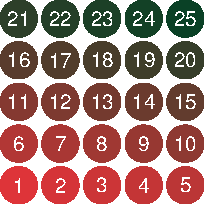
\includegraphics[scale=0.8]{scatter-color1}}\vss}

\newpage
\subsection{CMYK colours}

\MP\ also implements a CMYK colour model, using tuples of four numerics.  
This is more or less a direct mapping onto the PostScript "cmykcolor" functions.
In this model the four components represent cyan, magenta, yellow, and black.
White is \mpl{(0,0,0,0)} and black is anything where the last component is 1.
Beware however that the constants, \mpl{white} and \mpl{black} are defined in
"plain.mp" as RGB colours, and you can't mix the two models, so anything like 
\mpl{1/2[(1,1,0,0), white]} will not work.  If you want to do lots of work with CMYK colours
you might like to redefine the color constants.
$$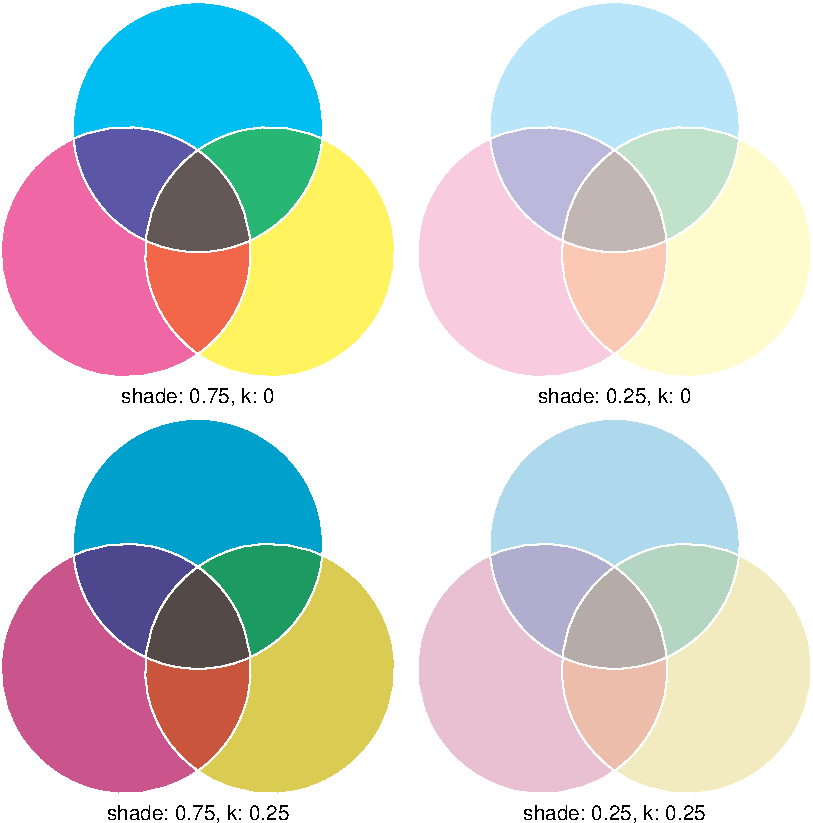
\includegraphics[width=0.7\textwidth]{color-wheel1}$$
Note that the apparent blending of colours here is done by calculating the overlaps
and filling them in order.  There is no support for transparency in any of the
colour models; this is because they are inherited directly from PostScript.  

\moveright 384pt\vbox to 0pt{\vss
\begin{code}
% the illusion of blended colours is helped by buildcycle

path C[], B[];

% arrange each circle so that point 0 is outside the others
C1 = fullcircle scaled 120 rotated 90 shifted 40 up;
C2 = C1 rotated 120;
C3 = C2 rotated 120;

B0 = buildcycle(C1, C2, C3);
B1 = buildcycle(C1, C2);
B2 = buildcycle(C2, C3);
B3 = buildcycle(C3, C1);

picture P;
for x=0 upto 1:
  for y=0 upto 1:
      P := image(
          s := 1/4 + x/2;
          k := 0 + y/4;
          fill C1 withcolor s*(1,0,0,k);
          fill C2 withcolor s*(0,1,0,k);
          fill C3 withcolor s*(0,0,1,k);
          fill B3 withcolor s*(1,0,1,k);
          fill B2 withcolor s*(0,1,1,k);
          fill B1 withcolor s*(1,1,0,k);
          fill B0 withcolor s*(1,1,1,k);
          undraw C1; undraw C2; undraw C3;
      ) shifted -(200x, 200y);
      draw P;
      label.bot(("shade: " & decimal s & ", k: " & decimal k)
                 infont "phvr8r", point 1/2 of bbox P); 
  endfor
endfor
\end{code}}

\newpage
\subsection{HSV colours}

HSV colours are colours defined by a triple of hue, saturation, and value.
Unlike RGB and CMYK colours there is no native support in \MP\ but it is possible to 
write a routine that maps HSV triples into RGB colours:
\begin{code}
vardef hsv_color(expr h,s,v) =
    save chroma, hh, x, m;
    chroma = v*s;
    hh = h/60;
    x  = chroma * (1-abs(hh mod 2 - 1));
    m  = v - chroma;
    if     hh < 1: (chroma,x,0)+(m,m,m)
    elseif hh < 2: (x,chroma,0)+(m,m,m)
    elseif hh < 3: (0,chroma,x)+(m,m,m)
    elseif hh < 4: (0,x,chroma)+(m,m,m)
    elseif hh < 5: (x,0,chroma)+(m,m,m)
    else:          (chroma,0,x)+(m,m,m)
    fi
enddef;
\end{code}
This is based on information from the Wikipedia article on 
on “HSL and HSV”.  

\medskip\noindent
The hue values in HSV colours map nicely to the familiar spectrum
of the rainbow.  In the model used here 0 is red, 120 green, and 240 blue:
$$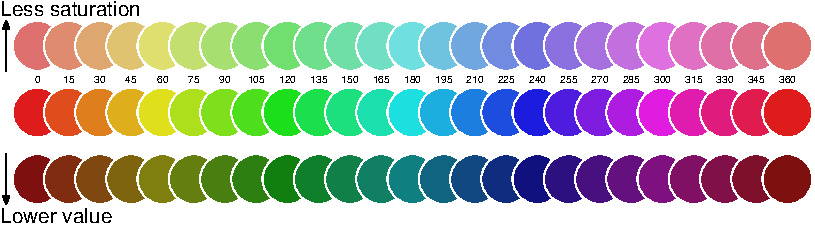
\includegraphics[width=0.85\textwidth]{hsv-samples1.pdf}$$
With less saturation the colours look faded; if you lower the value they get
darker.  Once you get the hang of them, they make choosing colours rather easier.
You can produce ranges of colour by changing hue, or make gradations of a single
colour by changing the saturation or value.

\moveright 384pt\vbox to 0pt{\vss
\begin{code}
defaultfont := "phvr8r";

numeric s[], v[];
s0 = 1/2; v0 = 7/8;
s1 = 7/8; v1 = 7/8;
s2 = 7/8; v2 = 1/2;
for y=0 upto 2:
  for h=0 step 15 until 360:
    fill fullcircle scaled 24 shifted (h, -32y) 
          withcolor hsv_color(h, s[y], v[y]);
    draw fullcircle scaled 24 shifted (h, -32y)
          withcolor white;
    if y=1: 
      label(decimal h infont defaultfont scaled 1/2, (h,-16)); 
    fi
  endfor
endfor

label.urt("Less saturation", (-20,12));
label.lrt("Lower value", (-20,-76));

drawarrow (-15, -12) -- (-15,12);
drawarrow (-15, -52) -- (-15,-76);
\end{code}}

\newpage
\subsection{An HSV example of a graduated scale}

\noindent
This example requires the \mpl{hsv_color} routine from the previous page.
\mpic{12pt}{hsv-samples2}
\begin{code}[xleftmargin=0pt]
defaultfont := "phvr8r"; defaultscale := 3/4;
path h,d,b; numeric n; n = 10;
h = ((-2,0)--(0,0)--(-1,3)--(-2,3)--cycle) scaled 60;
d = h rotated 180;
b = subpath (0,1) of h -- point 1+1/n of d -- 
    (xpart point 0 of h, ypart point 1+1/n of d) -- cycle;
fill b withcolor hsv_color(123, 1/8, 7/8);
draw subpath (2.13,4) of b;
for i=1 upto n:
    fill point 4-(i-1)/n of h -- point 1+(i-1)/n of h 
         -- point 1+i/n of h -- point 4-i/n of h -- cycle
         withcolor hsv_color(42, 1/4 + 3/4 * i/n, 1 - i/3n);
    fill point 4-(i-1)/n of d -- point 1+(i-1)/n of d 
         -- point 1+i/n of d -- point 4-i/n of d -- cycle
         withcolor hsv_color(200, i/n - 1/n, 1 - i/3n);
endfor
string s;
for i=1 upto n-1: 
    draw point 4-i/n of h -- point 1+i/n of h; 
    draw point 4-i/n of d -- point 1+i/n of d; 
    s := decimal if i < 4: (i**2+1) else: (10 + (i-3)*10) fi & "00";
    label.rt(s, point 1+i/n of h);
    label.lft(s, point 1+i/n of d);
endfor
label.rt("Metres", point 2 of h);
label.lft("Metres", point 2 of d);
label.lft("Hypsometric tints" infont defaultfont 
        scaled defaultscale rotated 90, point 7/2 of h);
label.rt("Bathymetric tints" infont defaultfont
        scaled defaultscale rotated -90, point 7/2 of d);
label.lft("sea level", point 0 of h);
label("areas below sea level", center b);
draw h; draw d;
\end{code}



\newpage
\subsection{Grey scale}

\moveright5.5in\vbox to 0pt{\vskip6pt
\begin{code}[xleftmargin=0pt]
numeric s; s = 13;
path atom; 
atom = origin 
   -- (2s,0) rotated -30 -- (2s,0) rotated -30 + (0,s)
   -- ( s,0) rotated  30 -- ( s,0) rotated  30 + (0,s)
   -- (0,2s) -- cycle;

picture p[];
for i=0 upto 2:
    p[i] = image(
        fill atom rotated -120i withcolor (7/8 - 1/8i) ;
        draw atom rotated -120i;
    );
endfor

n = 13;
for i=-n upto n:
    for j=-n upto n:
        forsuffixes $=0,1,2:
            draw p$ shifted ((3i*s,0) rotated -30 
                           + (0,floor(1/2i)*3s + 3j*s));
        endfor
    endfor
endfor
        
clip currentpicture to (unitsquare shifted -(1/2,1/2) 
                        xscaled 55.425s  yscaled 30s);   
\end{code}
\vss}
\noindent
The \mpl{withcolor} command will also take a single \mpl{numeric} instead of a 3-tuple or
a 4-tuple.  This produces a colour in grey scale (or gray scale if you prefer the
Webster spellings).  Just as for the other colour types, values below 0 count as
zero and values above 1 count as one.  And since the smallest possible positive
number in plain \MP\ is: $\id{epsilon} = 1/256/256;$ then you can have at most 65,536 shades in
between.

Grey scale is appropriate for some printed media, and can make effective textures
and patterns.
The code on the right was used to produce this:
$$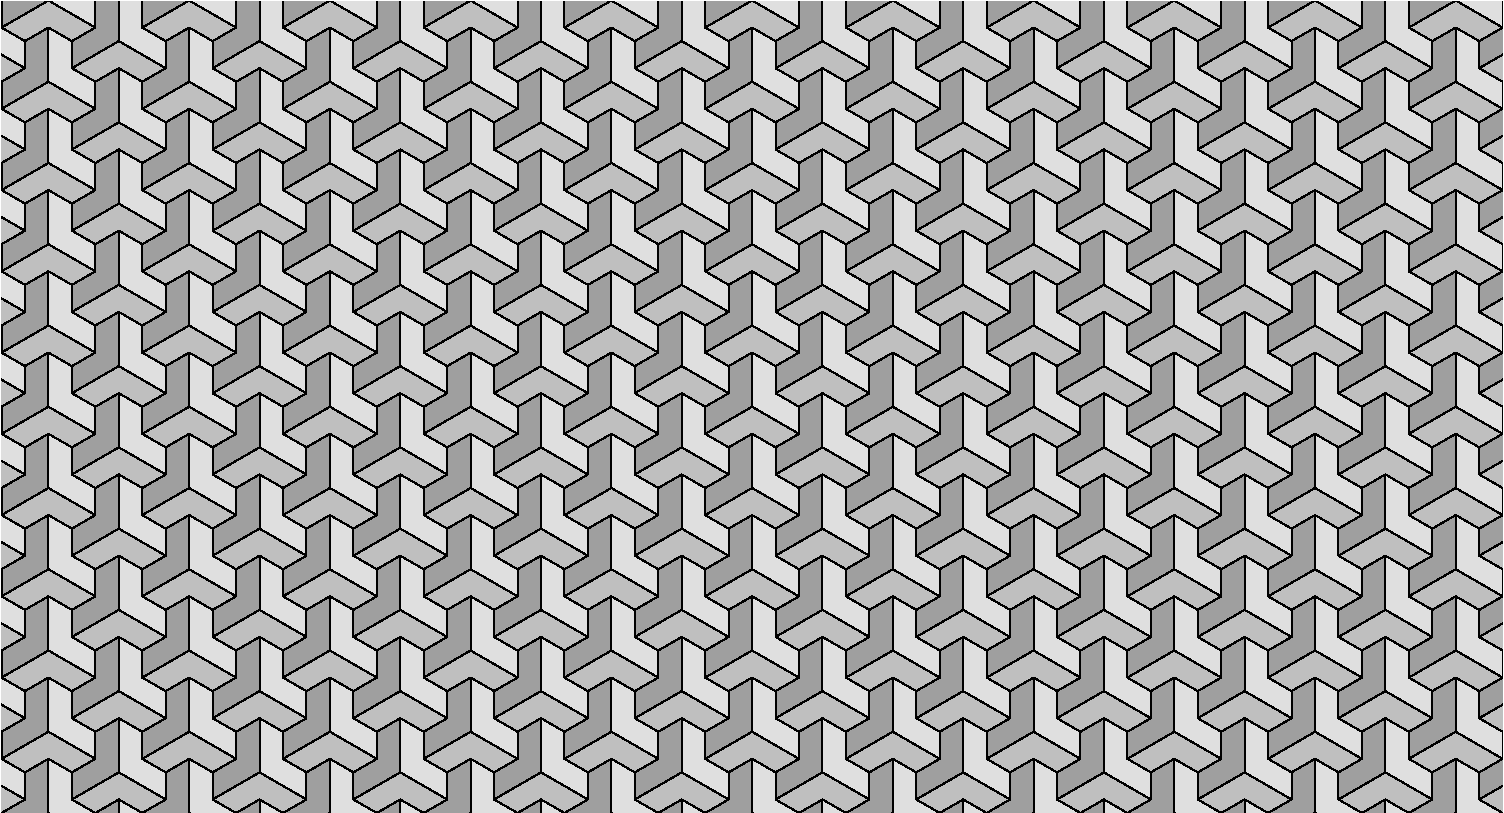
\includegraphics[width=\textwidth]{escher1}$$
First a basic path (named $\id{atom}$) is defined, then in the first loop three 
picture variables, $p_1$, $p_2$, and $p_3$, are defined, each one rotated
120° from the previous and filled with a slightly darker shade of grey.
The double loop then draws the three versions of the shape on an up-and-down grid.
Finally the picture is clipped to a neat rectangle.

\newpage
\subsubsection{Drawing algorithmic shadows}
\moveright5.5in\vbox to 0pt{\vskip6pt
\begin{code}[xleftmargin=0pt]
path b, w; 
b = ((-3,-4)--(3,-2)--(3,+2)--(-3,4)--cycle) scaled 5;
w = b reflectedabout(up, down);

numeric n;
n = 128;

picture B, W;
B = image(for i=0 step 1/n until 1: 
              draw point 4-i of b -- point 1+i**2 of b 
                  withcolor 1-i**8; 
          endfor);

    W = image(for i=0 step 1/n until 1: 
              draw point 4-i of w -- point 1+i**2 of w 
                  withcolor 3/4-i**8; 
          endfor);

for i=-9 upto 9:
    for j=-4 upto 4:
        draw if odd (i+j): W else: B fi shifted (i*30,j*30);
    endfor
endfor

clip currentpicture to bbox currentpicture yscaled 7/8; 
\end{code}
\vss}
\noindent
Here is a more complex pattern, showing one way to create an 
illusion of shadows with multiple fine lines.
$$
\includegraphics[width=\textwidth]{more-grey2}$$
The first part defines two wedge-shaped closed paths, $\id{w}$ being 
the mirror image of $\id{b}$.  Like the standard \id{unitsquare} path, the 
path $\id{b}$ is defined so that point 0 is the bottom left corner. 

The two $\kw{picture}$ variables are produced
by drawing lines across the shapes from bottom to top.  By setting $n$ high enough,
these multiple lines blend smoothly to give an even colour.  And by using higher
powers of the index variable, an effective shadow can be drawn ‘bunched up’ into the 
top of each shape.  

By repeating them alternately in a grid, we get an effective texture, which is
clipped at the end to a neat rectangle again.


\newpage
\subsection{Colorbrewer palettes}

The well-known Colorbrewer website ("http://colorbrewer2.org") provides a 
useful set of colour palettes that are suitable for a wide range of applications.  They 
were originally written for maps.  You can get my implementation of these palettes
for \MP\ from 
\begin{itemize}
    \item CTAN – "https://ctan.org/pkg/metapost-colorbrewer"
    \item Github – "http://github/thruston/metapost-colorbrewer"
\end{itemize}
The package provides two files that define all the colour ranges; one for CMYK and
another for RGB.  To use them you have to put them into your local TeX tree so that
\MP\ will find them.  On my Mac this means putting the files into
"~/Library/texmf/metapost".
\vadjust{\moveright 384pt\vbox to 0pt{\raggedright\hsize4in\vskip1in\noindent
The map shows the "RdYlBu[9]" palette in action on a map of the Brexit vote in
London.  The size of the circles represents the votes in each area, and the 
colours show how we voted.  The data is from publically-available UK
government sources.  The map was created with a small Python script to 
read the CSV files and write simple lines of \MP\ input.  You \textit{can} read
CSV files with \MP\ but it's much quicker with Python.

\begin{code}

    
\end{code}

\par\vss}}
$$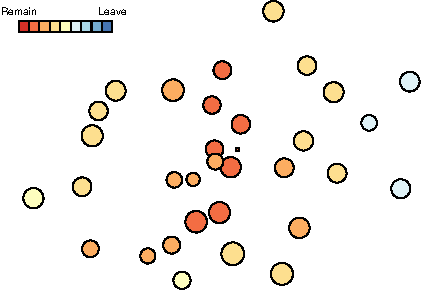
\includegraphics[width=\textwidth]{brexit-map.pdf}$$


\newpage
\section{Random numbers}

\MP\ provides us with two built-in functions to generate random numbers.
\vadjust{\moveright 384pt\vbox to 0pt{\kern-24pt
\begin{code}
vardef dice(expr pip_count, pip_color) = 
  save d,r,p, ul, ur, lr, ll; 
  r=1/8; path d; picture p;
  d = for i=0 upto 3: 
        quartercircle scaled 3 shifted (15,15) rotated 90i -- 
      endfor cycle;
  p = image(draw fullcircle scaled 6; 
            fill fullcircle scaled 6 withcolor pip_color);
  pair ul, ur, ll, lr;
  ul = 1/5[ulcorner d, lrcorner d];
  lr = 4/5[ulcorner d, lrcorner d];
  ur = 1/5[urcorner d, llcorner d];
  ll = 4/5[urcorner d, llcorner d];
  image(fill d withcolor background; draw d;
  if odd(pip_count):
     draw p shifted center d;
  fi;
  if pip_count > 1:
     draw p shifted ul; draw p shifted lr;
  fi;
  if pip_count > 3:
     draw p shifted ur; draw p shifted ll;
  fi;
  if pip_count = 6:
     draw p shifted 1/2[ul,ur];
     draw p shifted 1/2[ll,lr];
  fi)
enddef;

beginfig(1);
for i=0 upto 4:
  draw dice(1+floor uniformdeviate 6, red) 
       rotated (2 normaldeviate) 
       shifted (36i,0);
endfor
endfig;
\end{code}
        $$
\includegraphics{dice1}$$
\vss}}
\begin{itemize}
    \item `$\kw{uniformdeviate}\,n$' generates a random real number between $0$ and
        $n$.  
        
        Note that the $n$ is required.  It can be negative, in which case you get negative random
        numbers; or it can be zero, but then you just get $0$ every time. In other words the
        implementation generates a number $r$ such that $0\le r<1$ and then
        multiplies $r$ by
        $n$. 

        If you want a random whole number, use `$\kw{floor}$' on the result.
        So to simulate six-sided dice, you can use `$1+\kw{floor}\,\kw{uniformdeviate}6$'.

        If you use the new number systems, you should beware that the numbers
        generated will all be multiples of $1\over4096$, so $\kw{uniformdeviate}
        8092$ (for example) will generate even integers instead of random real
        numbers.  This `feature' is an accident of the way that the original rather
        complicated arithmetic routines have been adapted.

    \item `\kw{normaldeviate}' generates a random real number that follows the
        familiar normal distribution. The algorithm used is discussed in \textsl{The
        Art of Computer Programming}, section~3.4.1.  
        If you generate enough samples, the mean should
        be approximately zero, and the variance about 1. 
        The chance of getting a number between $-1$ and 1 is
        about 68\%; between $-2$ and 2, about 95\%.
        $$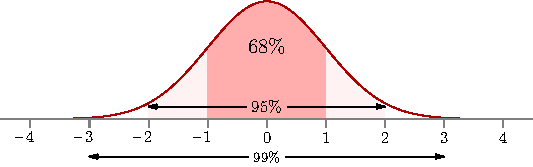
\includegraphics{gauss3}$$
        To relocate the mean, just add a constant.  To rescale the distribution, 
        multiply by the desired standard deviation (the square root of the
        desired variance).

    
\end{itemize}


\newpage\subsection{Random numbers from other distributions}

The \kw{normaldeviate} function is provided as a primitive \MP\ operation. The
implementation is based on the `Ratio method' presented in \textsl{The Art of
Computer Programming}, section~3.4.1.   It turns out to be very straightforward to
implement the algorithm for this method as a user-level program $\to$
\vadjust{\moveright5.5in\vbox to 0pt{\kern -64pt
\begin{smallcode}
vardef normaldeviate = 
    save u, v, xa; 
    forever:
        forever:
            u := uniformdeviate 1;
            exitif (u>1/64); 
        endfor
        v := sqrt(8/mexp(256)) * ( -1/2 + uniformdeviate 1 );
        xa := v/u; 
        exitif ( xa**2 <= -mlog(u)/64 );
    endfor
    xa
enddef;

vardef exponentialdeviate = 
  save u;
  forever: 
    u := uniformdeviate 1; 
    exitif (u>0); 
  endfor
  -mlog(u)/256
enddef;

vardef gammadeviate(expr a,b) = 
  save y, x, v, s, accept; boolean accept;
  s = sqrt(2a-1);
  forever:
    forever:
      y := tand(uniformdeviate 180);
      exitif y<64;
    endfor
    x := s * y + a - 1;
    accept := false;
    if x>0:
       v := uniformdeviate 1;
       if (v <= (1+y**2)*mexp((a-1)*mlog(x/(a-1))-(256*s*y))):
         accept := true;
       fi
    fi
    exitif accept;
  endfor
  x/b
 enddef;
\end{smallcode}
\vss}}%

There are a couple points here.  First, the inner loop around the assignment to $u$ is
designed to avoid very small values that would cause $v/u$ to be larger than 64, and
hence make "xa**2" overflow. This is a useful general technique, and justified in
terms of the algorithm since large values of $v/u$ are rejected anyway.  Secondly,
the expression "sqrt(8/mexp(256))" is a constant ($ \sqrt{8/e} \simeq 1.71553 $) and could be
replaced by it's value, but this does not make an appreciable improvement to the
speed of the routine.  On a modern machine, this routine is only very slightly
slower than using the primitive function.

It is also fairly straightforward to implement random number generators that follow other statistical
distributions.  The mathematical details are in the section of \textsl{TOACP}
referenced above. Two examples, for the exponential distribution and the gamma
distribution, are shown on the right.  In both cases note the care required to avoid
arithmetic overflow (and see section~\ref{trig} for the "tand" function). 

\medskip\noindent
You can also see the special nature of \MP's \kw{mexp} and \kw{mlog}
functions. They are defined so that $\kw{mexp} x = \exp(x/256)$ and $\kw{mlog} x =256\log(x)$.
This is another artefact of the scaled number system.  \MP\ computes $x^y$ using the
formula "mexp(y*mlog(x))", and the adjusted log values give more accurate results.

\medskip\noindent
At the start of each job, \MP\ automatically sets a new seed for the random number
generator, so that the sequence of numbers is different each time.  But you can set
this yourself if you need the same sequence each time.  At the start of your program
you should put "randomseed:=3.14;" (or whatever value you prefer). According to
\textsl{The Metafont Book}, the default value is
$\id{day}+\id{time}\ast\id{epsilon}$, but in \MP\ the exact value used depends on
the resolution of the timers available on your system.  


\newpage\subsection{Random walks}

You can use the random number generation routines to produce visualizations of
random walks, with various levels of analysis.
\vadjust{\moveright5.5in\vbox to 0pt{\kern -2\baselineskip
\begin{code}
beginfig(1);
w = 377; h = 233; n = 500;
pair zenith, nadir; zenith = nadir = origin;
path walk[];
for i=1 upto 16:
  y := 0;
  walk[i] = origin for x=0 step w/n until w: 
     hide(
       d := floor uniformdeviate 2 * 2 - 1;
       y := y + d;
       if y > ypart zenith: zenith := (x,y) ; fi
       if y < ypart nadir:  nadir  := (x,y) ; fi
     ) 
     -- (x,y) 
  endfor;
  draw walk[i] withcolor ((y+h/4)/(h/2))[red,blue];
  endfor

draw (origin--right) scaled w;
draw (origin--right) scaled w shifted (0,+h/4) withcolor 3/4;
draw (origin--right) scaled w shifted (0,-h/4) withcolor 3/4;

drawarrow (12 up   -- 2 up  ) shifted zenith withcolor blue;
drawarrow (12 down -- 2 down) shifted nadir  withcolor red;

endfig;
\end{code}
\vss}}
$$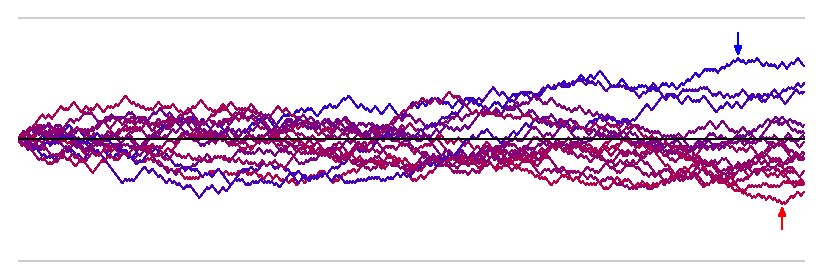
\includegraphics[width=\textwidth]{brown2}$$
In this example the random walk lines are coloured according to the final $y$-value,
and the global maximum and minimum points are marked.

Each walk is created with an `inline' for-loop; the loop is effectively expanded
before the assignment, so that each \id{walk} variable becomes a chain of connected $(x,y)$
pairs.  Inside the loop you can conceal yet more instructions in a `\kw{hide}' block.
These instructions contribute nothing to the assignment, but can change the values
of variables outside the block.

Note the first line of the \kw{hide} block sets "d" to $-1$ or $+1$. 
You can (of course) create different kinds of random walks, by changing the way you
set this delta value, for example by removing the \kw{floor} instruction, or scaling
the value, or changing the odds in favour of one direction or the other.  For
example:
$$d\gets\null\kw{if}\ p > \kw{uniformdeviate}\ 1: +1 \:\kw{else}: -1 \kw{fi};$$
will set $d$ positive with probability $p$ and negative with probability $1-p$.

\newpage\subsection{Brownian motion}

A random walk is normally constrained to move one unit at a time, but if you relax
that constraint and use `\kw{normaldeviate}' in place of `\kw{uniformdeviate}' you
can get rather more interesting patterns.\vadjust{\moveright5.5in\vbox to 0pt{
\hsize4in\kern -20pt
\begin{code}
beginfig(2);
for n=1 upto 4:
  x:=y:=0;
  draw (x,y) for i=1 upto 2000: 
    hide(x:=x+4normaldeviate; y:=y+4normaldeviate;) 
    .. (x,y) 
  endfor withcolor ((n+2)/9)[blue,white];
  fill fullcircle scaled 3 shifted(x,y) withcolor red;
endfor
% mark the origin
fill fullcircle scaled 3 withcolor green;
endfig;
\end{code}

\kern 120pt
\noindent
One of the features of using these random number generators is that the output is
different each time because \MP\ produces a different sequence of numbers.  You may
find yourself running the program a few times until you find one you like. At this
point you will wish that you knew what "randomseed" had been used, so that you can
re-create picture.  Unfortunately \MP\ does not log the value unless you set it
manually.  So here's a trick to use in this situation: set your own random seed
using a random number at the top of your program.
\begin{code}
    randomseed := uniformdeviate infinity;
\end{code}
Now you will find \MP\ writes the value it used in the log.
\vss}}
If you also allow the $x$-coordinates to
wander at random as well as the $y$-coordinates you get two-dimensional random
patterns.  And if you replace the straight line segments "--" with ".." so that \MP\
draws a smooth curve through the points, as well as vary the colour each time
you draw a new curve, then the result is almost artistic.

\medskip\noindent
\hbox to \textwidth{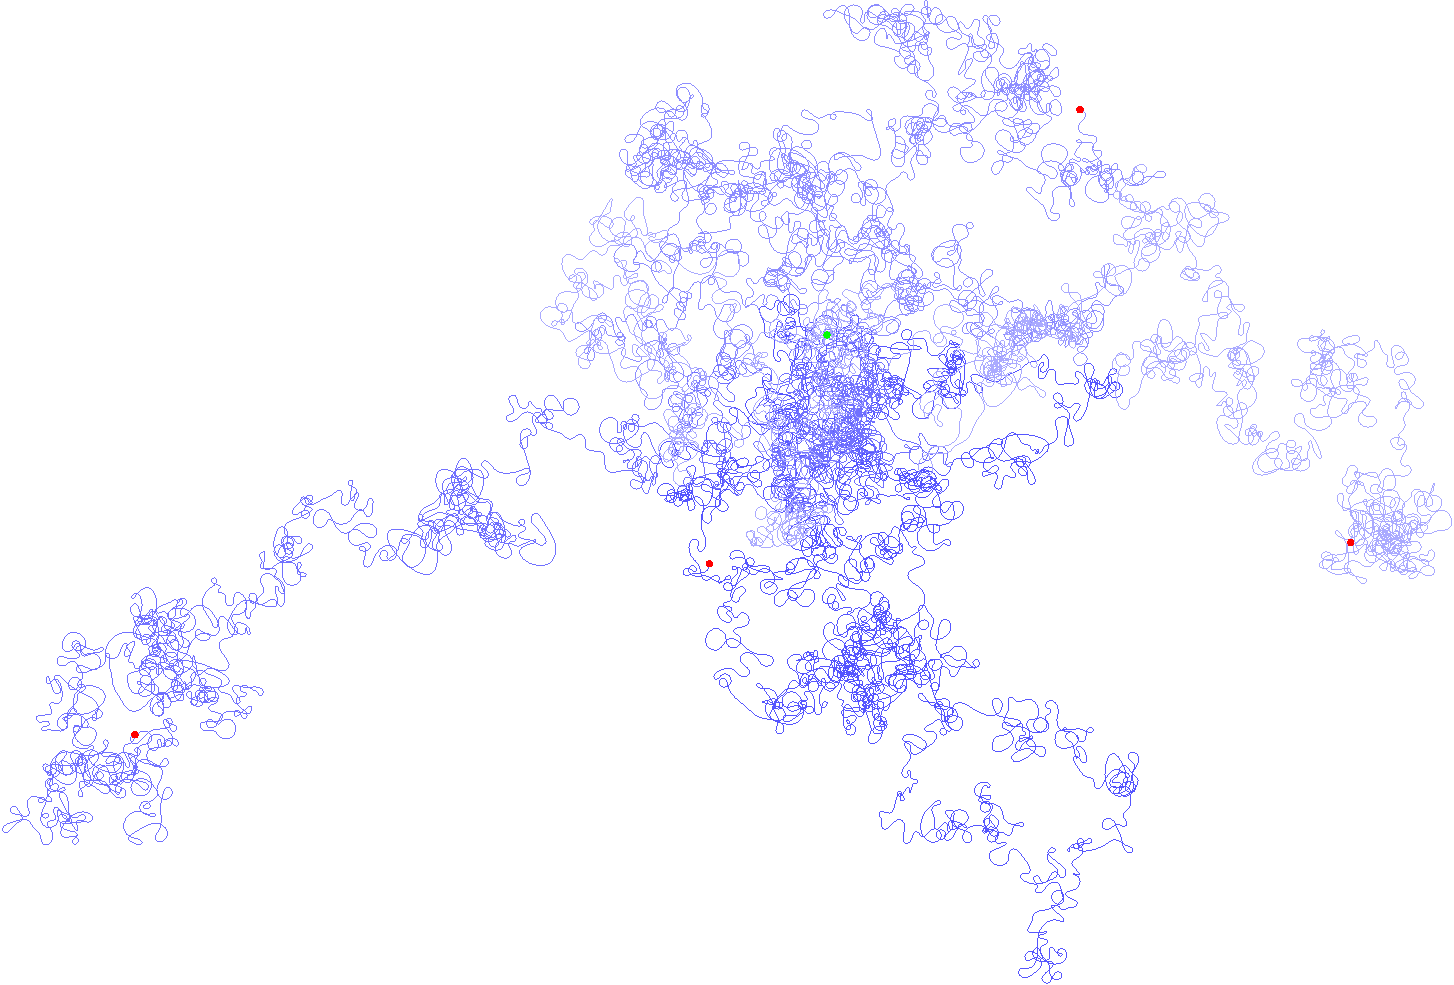
\includegraphics[width=1.2\textwidth]{brown3a}\hss}

\newpage\subsection{Drawing freehand}

This idea is shamelessly stolen from the wonderful collection of \MP\ examples
available at "http://melusine.eu.org/syracuse/metapost/".  But since the
examples there are all in French (including all the names of the custom macros), 
perhaps it would be better to say `translated' rather than `stolen';  moreover my
implementations are easier to use with plain \MP.\vadjust{\moveright5.5in\vbox to 0pt{
\hsize4in\kern -5.5\baselineskip
\begin{smallcode}
defaultfont := "eurm10";

def freehand_segment(expr p) =
  point 0 of p {direction 0 of p rotated (4+normaldeviate)} .. 
  point 1 of p {direction 1 of p rotated (4+normaldeviate)}
enddef;

def freehand_path(expr p) = 
  freehand_segment(subpath(0,1) of p)
  for i=1 upto length(p)-1:
    & freehand_segment(subpath(i,i+1) of p)
  endfor
  if cycle p: & cycle fi
enddef;

picture mark[];
mark1 = image(draw (left--right) scaled 2 rotated 60);
mark2 = image(draw mark1 shifted left; draw mark1 shifted right);

def moved_along expr x of p = rotated angle direction x of p 
                              shifted point x of p enddef;

z0 = (0,-1cm); z1 = (6cm,0);  z2 = (4cm,3cm); 
path t, c; 
t = freehand_path(z0--z1--z2--cycle);
c = freehand_path(z0..z1..z2..cycle);

z3 = point 1/2 + 1/20 normaldeviate of subpath (0,1) of t;

beginfig(1);
draw c withcolor .67 red;
draw t;
draw freehand_segment(point 2 of t--z3);
draw mark2 moved_along 1/4 of t;
draw mark2 moved_along 3/4 of t;

label.lft("A", z0);
label.rt ("B", z1);
label.top("C", z2);
label.bot("D", z3);
endfig;
\end{smallcode}
\vss}}

\subsubsection{Making curves and straight lines look hand drawn}

$$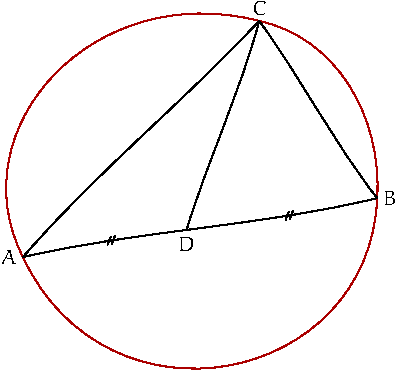
\includegraphics{freehand1}$$
A small amount of random wiggle makes the drawing come out charmingly wonky.  Notice
that the "freehand_path" macro will transform a path whether it is straight or curved,
and open or cyclic.  Notice also that to find the mid-point of a line, you find the
point along the freehand path; if you simply put "1/2[a,b]" there's no guarantee
that the point would actually be on the free hand path between "a" and "b".  In this
case a little extra randomness has been added, and the 
two segments $AD$ and $DB$ have been marked with traditional
markers to show that they are equal.  The "moved_along" macro combines shifted and
rotating to make the markers fit the wonky lines properly.
The Euler font complements the hand-drawn look;
you might find that a little of this type of decoration goes a long way.

\newpage\subsubsection{Extending straight lines slightly}

This second freehand figure uses the same macros as the one on the previous page,
but now the ink colour is set to sepia, and the lines are given a slightly more hand
drawn look at the corners.\vadjust{\moveright5.5in\vbox to 0pt{
\hsize4in\kern -3\baselineskip
\begin{code}
color sepia; sepia = (0.44, 0.26, 0.08);

def draw_out(expr p, o) = 
  draw p;
  for i=1 upto length(p):
     draw (unitvector(direction i-eps of p) scaled +o 
           -- origin --
           unitvector(direction i+eps of p) scaled -o) 
           shifted point i of p;
  endfor
enddef;

def angle_label_pos(expr p, i, s) = 
  ( unitvector(point i-1 of p-point i of p)
  + unitvector(point i+1 of p-point i of p)
  ) scaled s shifted point i of p
enddef;

beginfig(2);
  drawoptions(withcolor sepia);
  draw_out(t,6);
  drawoptions(withcolor .78 blue);
  label.lrt ("a", point 1/2 of t);
  label.urt ("b", point 3/2 of t);
  label.ulft("c", point 5/2 of t);

  drawoptions(withcolor .67 red);
  label(char 11, angle_label_pos(t,2,10));
  label(char 12, angle_label_pos(t,0,14));
  label(char 13, angle_label_pos(t,1,10));
endfig;
\end{code}
\vss}}

$$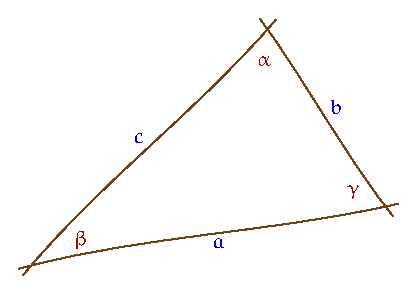
\includegraphics{freehand2}$$

\vfill
\nb\label{eulertable}
The AMS Euler font available to \MP\ as "eurm10" is encoded as a subset of the \TeX\
math italic layout --- essentially it has all the Greek letters but none of the
arrows.
$$
\includegraphics{freehand3}$$

\newpage\subsection{Increasingly random shapes of the same size}

If you want a random-looking shape, the general approach is to find a method to make
a path that allows you to inject some random noise at each point of the path.
$$\hbox to \textwidth{
\includegraphics{random-simple2}\hss}$$
For these shapes the objective was to make them increasingly random, but to keep
them all the same length.\vadjust{\moveright5.5in\vbox to 0pt{
\hsize4in
\begin{code}
beginfig(1);
desired_length := 180; n := 30; s := 80;
path shape;
for r=0 upto 8:
  shape := for i=0 upto n-1: 
             (s + r * normaldeviate, 0) rotated (360/n*i) ..
           endfor cycle;
  shape := shape scaled (desired_length/arclength shape);
  shape := shape shifted (r*s,0);
  draw shape withcolor (r/8)[black,red];
  label(decimal r, center shape);
endfor
endfig;
\end{code}
\vss}}
The basic path was a circle with radius "s" drawn by a loop with "n" steps like
this:
\begin{code}
for i=0 upto n-1: (s,0) rotated (360/n*i) .. endfor cycle
\end{code}
The random noise is then added to the $x$-coordinate at each step: when the noise is
zero ($\id{r}=0$) you get a circle; as the noise increases the circle is
increasingly distorted.  

The scaling is done using the "arclength" operator.  This works like "length" but
instead of telling you the number of points in a path, it returns the actual length
as a dimension.  Dividing the desired length by this dimension gives the required
scaling factor for the random shape just defined.

Note that since we assign to "shape" each time round the loop, we have to use ":="
to update the value instead of "=".

\newpage\subsection{Explosions and splashes}

Random numbers are also useful to make eye catching banners for posters,
presentations, and infographics.  Here are two simple example shapes: $\to$
\mpic{18pt}{explode1}

\begin{smallcode}
string heavy_font; 
heavy_font = "PlayfairDisplay-Black-osf-t1--base";

randomseed:=2128.5073;

beginfig(1);  
n = 40; r = 10; s = 50;
path explosion, splash;
explosion = for i=1 upto n:
  (s if odd(i): - else: + fi r + uniformdeviate r,0) rotated (i*360/n) --
endfor cycle; 

splash = for i=1 upto n:
  (s if odd(i): - else: + fi r + uniformdeviate r,0) rotated (i*360/n) ..
endfor cycle; 
splash := splash shifted (3s,0);

fill explosion withcolor 1/2 green + red;
draw explosion withpen pencircle scaled 2 withcolor 2/3 red;
label("BOOM!" infont heavy_font scaled 2, center explosion)
                                                     withcolor red;
fill splash withcolor 1/2 green + blue;
draw splash withpen pencircle scaled 2 withcolor 2/3 blue;
label("SPLAT!" infont heavy_font scaled 2, center splash) 
                                                     withcolor blue;
endfig;
\end{smallcode}

\noindent
In this figure "n" is the number of points in the shape, "r" is the amount of
randomness, and :"s" is the radius used.
In order to get a clear zig-zag outline, the loop alternately adds or subtracts "r";
and then adds a random amount on top to make it look random.
Notice that the only difference between the "explosion" and "splash" is that how
the connecting lines are constrained to be straight or allowed to make smooth
curves.\vadjust{\moveright5.5in\vtop to -2pt{\hsize 4in\vss\noindent 
The display font used here is one of the gems hidden away in "psfonts.map".
If you run \MP\ with the "-recorder" option, it will create a list of all the files
used, with the current job name and an extension of ".fls".  This file will include
a line which tells you exactly which version of "psfonts.map" is being used.  

The DVIPS documentation explains the format of the file, but for \MP's purposes the
first word of each non-comment line defines a font name you can try.  However beware
that just because a name is defined in your map file, does not necessarily mean that
you actually have the required PostScript font files installed as well.  But if you have a
full TexLive installation you will find that very many of them are already
installed.\strut
}}


\newpage\subsection{Simulating jagged edges or rough surfaces}

You can use the idea of adding a little bit of noise to simulate a rough surface.
$$
\includegraphics{qed1}\quad
  
\includegraphics{qed2}$$
These diagrams are supposed to represent light rays reflecting from a surface: on
the left the surface is smooth ($r=0$) and on the right it's rough ($r=0.42$).  
The parameter $r$ is used in the \MP\ program as a scaling factor for the random
noise added to each point along the rough surface; the only difference in the code
to produce the two figures was the value of $r$.%
\vadjust{\moveright5.5in\vbox to
    0pt{\hsize 4in\vss
\begin{smallcode}
def perpendicular expr t of p = 
  direction t of p rotated 90 shifted point t of p
  enddef;

beginfig(1);
u = 5mm;  r = 0.42; n = 32; s = 8u; theta = -45;

path base;
base = origin 
       for i=1 upto n-1: -- (i/n*s,r*normaldeviate) endfor 
       -- (s,0) -- (s,-u) -- (0,-u) -- cycle;
fill base withcolor .8[blue,white];
draw base withcolor .67 blue;

path ray[];
for i=2 upto 6:
  ray[i] = (left--right) scaled 2/3 s rotated theta shifted (i*u,0);
  b := ypart (ray[i] intersectiontimes base);
  ray[i] := point 0 of ray[i] 
         -- point b of base 
         -- point 0 of ray[i] 
            reflectedabout(point b of base, perpendicular b of base);
  drawarrow ray[i];
endfor   

label("r=" & decimal r, center base);
endfig;
\end{smallcode}
\vss}}
First the base block is created with some noise on the upper side.  Then five rays
are created.  Applying \mpl{ypart} to the pair of times returned by
\mpl{intersectiontimes} gives us the point of the base where the incident ray hits
it.  This point and the perpendicular at that point are then used to get the angle
for the reflected ray.  The diagrams are effective because the rays are reflected at
realistic looking angles.

The simple approach to adding noise along a path works well in most cases provided
there's not too much noise,  but it is always possible that you'll get two consecutive
values at opposite extremes that will show up as an obtrusive jag in your line.  To
fix this you can simply run your program again to use a different random seed value;
or you could try using ".." instead of "--" to connect each point, but beware that
sometimes this can create unexpected loops.  

\newpage\subsubsection{Walking along a torn edge}

It's also possible to use a random
walk approach so that each random step takes account of the previous one to avoid
any big jumps.  Here's one way to do that.
\begin{code}
beginfig(1);
  y=0;
  path e; 
  e = (0,y) for i=1 upto 288: -- (i,walkr y) endfor ;
  draw e;
endfig;  
\end{code}
$$
\includegraphics{torn-edge1}$$
The "walkr" routine works like the "incr" and "decr" commands; it updates the value of the
argument.  The idea is that the further away from zero you are, the more likely is
that the next value will take you back towards zero.  
\begin{code}
vardef walkr suffix $ = 
  $ := $ if uniformdeviate 1 < (2**-abs($)): + else: - fi 
    signr $; $ 
  enddef;
vardef signr suffix $ = 
  if $<0: - else: + fi uniformdeviate 1 
  enddef;
\end{code}
You can use this to produce more realistic torn edges.  You can also apply this as a
form of jitter to a curved path, by adding a suitably rotated vector to enough
points along the path.

\moveright5.5in\vbox to 0pt{\kern-4in
\begin{code}
beginfig(2);
path c; c = fullcircle scaled 200;
draw c withcolor .8 white;

y=0; n = 600;
path t; t = for i=0 upto n-1:
  point i/n*length(c) of c 
  + (0, walkr y) rotated angle direction i/n*length(c) of c
  -- 
endfor cycle;
draw t withcolor .67 red;
endfig;
end.
\end{code}
$$
\includegraphics{torn-edge2}$$
\vss}


\newpage
\section{Plane geometry and trignonometry}

\noindent\vadjust{\moveright5.5in\vbox to 0pt{\hsize4in\kern-9pt\noindent
Here is the equilateral triangle point macro in action.

\begin{code}
beginfig(1);
path c; c = fullcircle scaled 144;
pair a,b,p,q;
for i=0 upto 7:
  a := point i   of c;
  b := point i+1 of c;
  p := equilateral_triangle_point(a,b);
  q := equilateral_triangle_point(b,a);
  draw a -- p -- b withcolor .67 green;
  draw a -- q -- b withcolor .67 red;
endfor
draw c withcolor .53 blue;
endfig;
\end{code}

$$\includegraphics{geometry3}$$
\vss}}%
This section deals with drawing geometrical figures typically involving lines,
angles, polygons, and circles.  Plain \MP\ provides very few tools that are
explicitly designed to help draw geometric figures, but it is usually possible to
find an elegant construction using these tools and the relevant primitive commands.
It is tempting to build up your own library of special purpose macros, but
experience suggests that it is often better to adapt a general technique to the task
in hand, and to create a specific solution to your current problem.  One of the main
issues is catching exceptions; since it is hard to write completely general macros,
the techniques presented here should be adapted as required rather than blindly
copied.

The classical constructions from Euclid's \textsl{Elements} are often useful 
sources of inspiration for macros, but they do not always point in the right 
direction.  For example consider the first proposition: \textit{given two points
find a third point, so that the three points make an equilateral triangle}.
Euclid's construction is to draw an arc, with radius equal to the length of the
segment between the two points, at each point and find the intersection.  This might 
lead us to a function like this:
\begin{code}
vardef equilateral_triangle_point(expr a, b) =
  save c; path c; c = fullcircle scaled 2 abs(b-a); 
  (c shifted a intersectionpoint c shifted b)
enddef;
\end{code}
This works but has a couple of issues.  First \mpl{intersectionpoint} is a bit slow and
not very accurate (although this might not matter to us); secondly and more
seriously, the point returned depends on the orientation of the points "a" and 
"b".  In some configurations the first intersection found will be on the left, in
others on the right.  We could fix this by rotating the circle "c" by "angle (b-a)",
but we can do better with a simple rotation of the second point about the first:
\begin{code}
vardef equilateral_triangle_point(expr a, b) =
  b rotatedabout(a,60)
enddef;
\end{code}
And if you want to get right back to primitives you could even write that as:
\begin{code}
vardef equilateral_triangle_point(expr a, b) =
  b shifted -a rotated 60 shifted a
enddef;
\end{code}

\newpage
\subsection{Bisecting lines and paths}

\moveright5.5in\vbox to 0pt{\hsize4in\noindent
        $$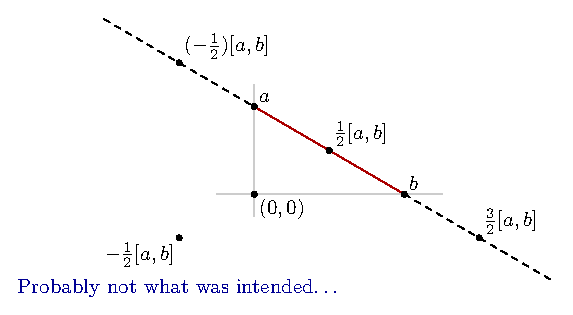
\includegraphics{mediation1}$$
        \vskip 50pt
        $$
\includegraphics{mediation2}$$
        \bigskip
        $$\includegraphics[width=4in]{mediation3}$$
        \centerline{Lee Sallows' theorem of median triangles}
\vss}
\noindent
The best way to bisect a line, depends on how you have defined it.
If you have two pairs $a$ and $b$, then the simplest way to find 
the pair that bisects them is to write "1/2[a,b]".  This mediation 
mechanism is entirely general, so you can write \mpl{1/3[a,b]}, "1/4[a,b]", and
so on to define other pairs that are part of the way from $a$ to $b$.
The expression "0[a,b]" is equal to $a$, and "1[a,b]" is equal to $b$;
but the number before the left bracket does not have to 
be confined to the range $(0,1)$.  If you write "3/2[a,b]" you will get a pair on
the extension of the line from $a$ to $b$ beyond $b$.  To get a pair going the
other way you can either reverse $a$ and $b$, or use a negative number; but don't
get caught out by the \MP\ precendence rules:  "-1/2[a,b]" is interpreted as
"-(1/2[a,b])" and not as "(-1/2)[a,b]", so either put in the parentheses or swap
the order of the pairs: "(3/2)[b,a]". See $\longrightarrow$.

If you want to work with a \kw{path} variable, rather than separate \kw{pair}
variables, you can 
use the \mpl{point t of p}
notation to do mediation along the path.  For a simple straight path $p$ of length 1
then \mpl{point 1/2 of p} will give you the midpoint.  More generally, 
\mpl{point 1/2 length p of p} will give you the midpoint of a path of any length. 
This works fine for simple paths, along which \MP's time moves evenly, 
but for more complicated, curved paths you have to use this rather cumbersome notation:
\begin{code}
    point arctime 1/2 arclength p of p of p
\end{code}
If your path is cyclic, and makes a triangle or a regular polygon,
then you can bisect it with the line 
\begin{code}
    point t of p -- point t + 1/2 length p of p
\end{code}
\textbf{NB}: if the polygon has an odd number of sides, then $2t$ must be a whole
number. 

\smallskip\noindent
In a triangle these bisecting lines are called medians.  The three medians intersect
at the centroid of the triangle.  The centroid is a good place to put a label on a
triangle.  You could find it \mpl{intersectionpoint} or with
a construction using \mpl{whatever} on any two medians, but since we know that the centroid
divides each median in the ratio $2:1$ we can find the centroid of a triangle path
$p$ most simply with:
\begin{code}
    z0 = 2/3[point 0 of p, point 3/2 of p];
\end{code}
The median is the basis for several beautiful theorems about the geometry of the
triangle. The theorem shown here was first published in 2014.

\newpage
\subsection{Bisecting angles}
\moveright5.5in\vbox to 0pt{\hsize4in\noindent
\begin{code}
vardef euclidean_bisector(expr a,b,c,r) = 
  save arc,p,q,e; 
  path arc; pair p,q,e;
  arc = fullcircle scaled r shifted b;
  p = (a--b) intersectionpoint arc;
  q = (b--c) intersectionpoint arc ;
  e = equilateral_triangle_point(p,q);
  e
enddef;
\end{code}
$$
\includegraphics{bisection1}$$
\begin{code}
vardef vector_bisector(expr a,b,c,r) = 
   b + unitvector (a-b) scaled r 
     + unitvector (c-b) scaled r
enddef;
\end{code}
$$
\includegraphics{bisection2}$$
\vss}
\noindent
In an equilateral triangle the medians also bisect the angles at each vertex; this
is the basis of Euclid's method of bisecting an angle set out in the Second
Proposition.  You can do the same in \MP, but it might not always be the best way.
Whatever approach you take, an angle is defined by three points; one that defines
the corner and two that define the lines extending from that corner.  In this
exploration I've used $a$, $b$, and $c$ to represent the points, with $b$ being the
one in the middle, and at the corner.

Euclid's method is to draw an arc centred at the corner, and then construct an
equilateral triangle on the two points where the arc crosses the lines. This is
shown on the right, with a macro that re-uses the equilateral triangle point macro
given above.  But if your aim were to find any point on the line bisecting $\angle
ABC$, then you could simplify this and make it more efficient by using
$e = \frac12[p,q]$
instead of calling the triangle macro at all.  However the macro is still making two
calls to \mpl{intersectionpoint}.  If you wanted to eliminate this you could use the 
useful plain \MP\ macro "unitvector" to produce a solution based on adding two equal
length vectors from the corner to the two other points.  Another approach is to
exploit another geometric theorem that states that the bisector of an angle in a
triangle divides the opposite side in the ratio of the two other sides. 
So if sides $AB$ and $BC$ have lengths $p$ and $q$ then the bisector will 
be ${p\over p+q}={1\over1+q/p}$ from $A$ to $C$, and you can express this
simply using \MP's mediation syntax:
\begin{code}
vardef interior_bisector(expr a,b,c) = 
  (1/(1+abs(c-b)/abs(a-b)))[a,c]
enddef;
\end{code}

\vbox to 0pt{
$$
\includegraphics{bisection3}$$
\vss}
\newpage
\subsection{Trisections and general sections of angles}

There is no classical method to trisect an arbitrary angle, so you need to resort
to measuring and arithmetic in \MP.  If the angle is a given this is trivial:
\mpic{-12pt}{trisection-simple.pdf}
\begin{smallcode}
path ray;
numeric theta;
ray = origin -- 200 right;
theta = 42;
draw ray;
draw ray rotated 1/3 theta withcolor 2/3 red;
draw ray rotated 2/3 theta withcolor 2/3 red;
draw ray rotated theta;
dotlabel.llft("$0$", origin);
label("$\theta/3$", 72 right rotated 1/6 theta);
label("$\theta/3$", 72 right rotated 3/6 theta);
label("$\theta/3$", 72 right rotated 5/6 theta);
\end{smallcode}
But if you have only the coordinates of some points then you need to use the
\mpl{angle} primitive to measure the angle first; \mpl{angle} takes a \kw{pair}
argument and returns a numeric representing the angle in degrees measured clockwise
from the $x$-axis to a line through the origin and the point represented by the pair.
This definition means that if you have three points $A$, $B$, and $C$, then you can
measure $\angle ABC$ with \mpl{angle(C-B)-angle(A-B)}. Following the usual
convention this gives you the angle at $B$; if you list the points in clockwise
order you will get a positive result. If you don't care about the order, you 
can make this into a more robust macro:
\begin{smallcode}
vardef measured_angle(expr P, Q, R) = 
  (angle (P-Q) - angle (R-Q)) * turningnumber (P--Q--R--cycle) mod 360
enddef;
\end{smallcode}
The primitive \mpl{turningnumber} is explained on p.\thinspace 111 of \textsl{The
METAFONTbook}.  It takes a cyclic path and returns number of times that you would
turn through 360${}^\circ$ if you traversed the path.  We use this here to
negate the measured angle if necessary, so that you always get the interior angle.
The \mpl{mod 360} on the end ensures that the result is in the range $0 \le \theta <
360$.  Armed with a measured angle, all you then need is arithmetic.
\mpic{-160pt}{trisection-classical.pdf}
It might be possible to use the \id{solve} macro to simulate the Neusis construction 
(that allows you to measure a length) illustrated on the right, but measuring the
angles is rather easier.

\newpage 
\subsection{Intersections}

\moveright5.5in\vbox to 0pt{\hsize4in\noindent
\centerline{A puzzle square featuring some intersections}
$$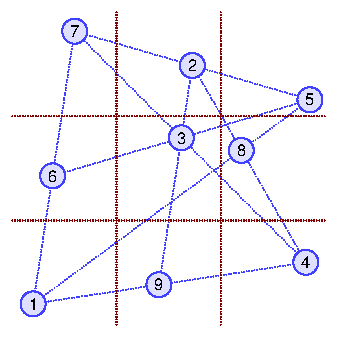
\includegraphics[width=3in]{magic-square-14}$$
The points were defined like this (the order was important).
\begin{code}
z1 = (10,10);
z4 = 144 right rotated 12;
z5 = z4 shifted (2, 78);
z7 = z4 reflectedabout(origin, (1,1));

z2 = 1/2 [z5, z7];
z9 = whatever [z1, z4];
z2-z9 = whatever * (z7-z1); 
z8 = whatever [z1, z5] = whatever [z2, z4];
z3 = whatever [z2, z9] = whatever [z4, z7];
z6 = whatever [z1, z7] = whatever [z3, z5];
\end{code}
\vss}
\noindent
If you have line segments defined by their endpoints, then the
canonical way to find their intersection, is to use
the mediation syntax with \id{whatever} twice:
$$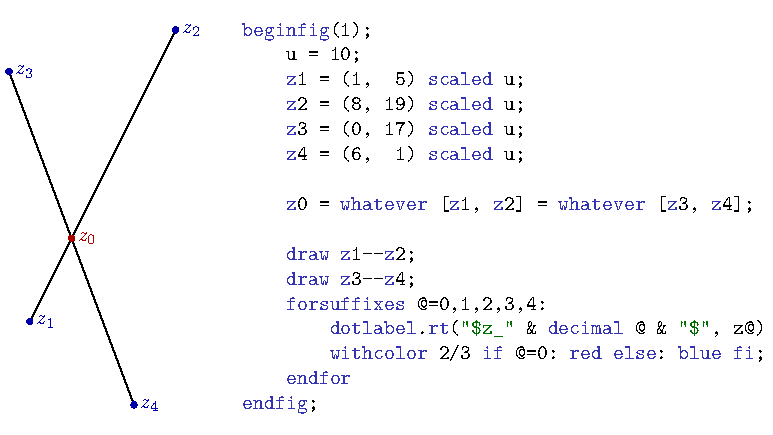
\includegraphics[width=0.9\textwidth]{whatever.pdf}$$
The mediation syntax works even if the interection point does not actually lie on
either of the two line segments.  The intersection will be the point where the two
(infinite) lines through the pairs of points meet.  If the two lines are parallel,
you'll get an `inconsistent equation' error.  If you want to capture the calculated
values, then use undefined numeric variables instead of \id{whatever}:
\begin{code}
    z0 = alpha [z1, z2] = beta [z3, z4];
\end{code}
In this example you would find $\alpha=0.286$ and $\beta=0.5$.
If you are trying to find where the line through your points intersects a horizontal or vertical, then you only need one
mediation and a simple equation for the relevant $x$ or $y$ coordinate:
\begin{code}
    z0 = alpha [z1, z2]; x0 = 0;  % for example
\end{code}
If you have defined your lines as paths, and especially if they are more complicated
than straight lines, you need to use the \mpl{intersectiontimes} primitive or the
\mpl{intersectionpoint} macro, as explained on pp.136–137 of \mfbook.

\newpage
\subsubsection{The intersection algorithm}

\MP\ inherits a fast algorithm for finding the intersection between two paths from
\MF.  It is explained rather more gnomically than usual at the end of Chapter 14 of
\mfbook, with more detail given in the web source for \MF.  The core algorithm works
on paths of length 1. If you have longer paths, \MP\ works its way along the paths
applying the core algorithm to successive pairs of unit subpaths.  It does this is
lexographic order; this means that, if you have two circles $A$ and $B$, and you do this:
\begin{code}
    (t, u) = A intersectiontimes B;
\end{code}
then \MP\ will first look for an intersection between subpath $(0,1)$ of $A$ and
subpath $(0,1)$ of $B$, then subpath $(0,1)$ of $A$ and subpath $(1,2)$ of $B$, and
so on, with $B$ varying faster, until you get to subpath $(7,8)$ of $A$ and subpath
$(7,8)$ of $B$.  But you may never get that far, as the process stops as soon as the
first intersection is found.  The upshot of this is that the intersection point
found will always be as early as possible on $A$.  Note that after the call above
point $t$ of $A$ will be very close to point $u$ of $B$, as they both refer to the
same intersection point.  If there is an alternative point that is earlier on $B$,
then use `$B \mathbin{\textrm{intersectiontimes}} A$' instead.\mpic{-222pt}{intersectme1} 
$$\vbox{\halign{$\vcenter{\hbox{#}}$&&\quad$\to\vcenter{\hbox{#}}$\cr
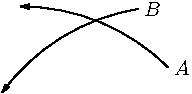
\includegraphics{intersectme0}&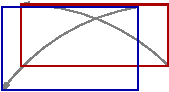
\includegraphics{intersectme2}&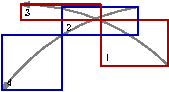
\includegraphics{intersectme3}\cr
}}$$
When we get down to paths of length 1, the core algorithm works as shown above.  The
two paths are represented as rectangles that enclose the end points and the control
points for each path.  If these rectangles don't overlap then there is certainly no
intersection. Otherwise \MP\ bisects each path and considers four smaller rectangles,
in the order $(1,2)$, $(1,4)$, $(3,2)$, $(3,4)$ (as shown above on the right).
It carries on doing this recursively (well actually using a stack to back track)
until it finds sufficiently small overlapping rectangles.  The two times returned by
\mpl{intersectiontimes} are the midpoints of these two tiny rectangles.
$$\vbox{\halign{$\vcenter{\hbox{#}}$&&\quad$\to\vcenter{\hbox{#}}$\cr
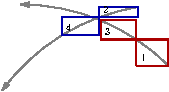
\includegraphics{intersectme4}&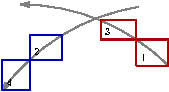
\includegraphics{intersectme5}&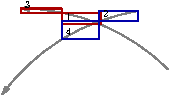
\includegraphics{intersectme6}&\quad$\cdots$\cr
}}$$


\subsubsection{Finding all intersection points}

As noted above, the \mpl{intersectiontimes} algorithm will stop at the first
intersection of the two paths, but it is possible that the two paths will intersect 
again further along.  If you want to find all the intersection points then the
simplest technique is just to unwrap the algorithm slightly, and loop through all
the unit subpaths applying \mpl{intersectiontimes} to each pair.  Using an array to
hold the points and a counter, you can get them with something like this:
\begin{smallcode}
pair P[], times; numeric n; n = 0;
for i = 1 upto length(A):
  for j = 1 upto length(B):
    times := subpath (i-1,i) of A intersectiontimes subpath (j-1,j) of B;
    if xpart times > -1:
      P[incr n] = 1/2[point xpart times of subpath (i-1,i) of A, 
                      point ypart times of subpath (j-1,j) of B];
    fi
  endfor
endfor
\end{smallcode}
and then use them like this:
\begin{smallcode}
for i=1 upto n:
    draw fullcircle scaled 4 shifted P[i]; % or whatever
endfor
\end{smallcode}
There are a couple of \MP\ technical points to note.  The \mpl{intersectiontimes}
operation returns a pair, which we assign to a pair variable $\id{times}$
above; we have to use \mpl{:=} to re-assign it in each loop, and we have to 
use an explicit pair variable because you can't assign to a literal pair;
\MP\ will give you an error if you try \mpl{(t, u) := A intersectiontimes B;}.
This may come as a surprise, because you \textit{can} legally do \mpl{(t, u) = A
intersectiontimes B}, but in a loop this causes an inconsistent equation error on
the second iteration.  If you need to avoid the repeated use of \mpl{xpart} and
\mpl{ypart}, one alternative is to do this inside the loop:
\begin{smallcode}
    ...
    numeric t, u;
    (t, u) = A intersectiontimes B;
    ...
\end{smallcode}
Now the numerics are reset each time and the equation is not inconsistent.
\vadjust{\moveright 384pt\vbox to 0pt{\hsize 4.2in\vss \noindent
T\textsc{he} technique discussed on the left, works well on paths where the points on one or
both of the paths are close together, so that the unit subpaths are short;
But it
is possible to create quite long paths of unit \mpl{length} and these may intersect
each other more than once, like so:
$$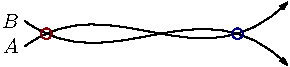
\includegraphics{intersectme8}$$
Here the two paths $A$ and $B$ are Bezier splines of with \mpl{length=1}, so the
normal \MP\ algorithm is only ever going to give you one of the intersections.  In
the diagram above, the
red circle marks the point given by \mpl{A intersectiontimes B}.  We can try
reversing one of the paths, and in this case you get the point marked in blue, 
but what about the one in the middle?

The most reliable approach is to take a copy of one of the paths, and snip it off at
the intersection and try again until there is nothing left to snip.
$$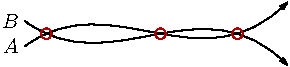
\includegraphics{intersectme9.pdf}$$
The three points marked here were captured like this:
\begin{code}
pair P[]; numeric n; n=0; 
path R; R := A;  % take a copy of A
forever:
  R := R cutbefore B;  % snip where we cross B
  exitif length cuttings = 0;  % stop if nothing was cut
  P[incr n] = point 0 of R; % capture the point
  R := subpath (epsilon, infinity) of R; % nudge along
endfor
\end{code}
This technique also works on paths with \mpl{length} greater than one, 
so you may prefer it as your general “get all the intersections” approach.
Note that the \mpl{cutbefore} macro is defined using \mpl{intersectiontimes}.

\kern 6.5pt
}}

\subsection{Parallel and orthogonal or whatever}

Given five known points --- $A$, $B$, $C$, $D$, and $E$ --- \MP\ can find the point $F$
on the line $A \to B$, so that $E \to F$ is parallel to $C \to D$ like this:
\mpic{0pt}{parallel1}
\begin{code}
    F = whatever[A, B]; % F is on the line A..B
    E-F = whatever * (C-D) % E..F || C..D
\end{code}
In the second line the expressions \mpl{E-F} and \mpl{C-D} return \mpl{pair}
variables and the equation with \mpl{whatever} says that they must be scalar
multiples of each other.  With the first equation, this is enough for \MP\ to work
out where $F$ should go.   Note that \mpl{whatever} can take any real value,
positive or negative, so it does not matter whether you put \mpl{E-F} or \mpl{F-E}.
Note also that for the same reason, while $F$ will lie on the line \textit{through}
$A$ and $B$, it might not lie on the segment from $A$ to $B$.

\smallskip\noindent\llap{\nb}%
To define a line perpendicular to $C\to D$ rather than parallel, you can write:
\begin{code}
    G = whatever[A, B];
    E-G = whatever * (C-D) rotated 90;
\end{code}
and obviously the "90" can be adjusted to whatever angle you please.

\smallskip\noindent\llap{\nb}%
If you need to compute the perpendicular distance from the point $C$ to a line $A\to
B$, you can use Knuth's ‘slick’ formula:
\begin{code}
    abs ypart ((C-A) rotated -angle (B-A))
\end{code}
This effectively rotates $C$ about $A$ by the angle of the line, so that the problem
is reduced to measuring the height of a point above the $x$-axis, which is what
\mpl{ypart} does, of course.

\smallskip\noindent\llap{\nb}%
There are some limitations to what you can do with \MP's linear equations; for one
thing you can't generally say things like \mpl{length(C-A) = 72}.  If you want to
find the two points on a line that are a given distance from an external point, it's
often simpler to find the intersection points of the line with a suitably scaled and
shifted circle, even if you don't actually then draw the circle.  You can usually
find the other point by reversing the circle.



%unitvector
%dotprod
%abs
%++ and +-+


%transformations

%- reflectedabout
%- rotatedaround

\newpage 
\subsection{Circle through three points}

\begin{code}
vardef circle_through(expr A, B, C) = 
    save m, n, o; pair m, n, o;
    m = 1/2[A,B]; n = 1/2[B,C];
    o = whatever[A rotatedabout(m, 90), B rotatedabout(m, 90)]
      = whatever[B rotatedabout(n, 90), C rotatedabout(n, 90)];
    fullcircle scaled 2 abs(A-o) shifted o
enddef;
\end{code}


\newpage
\subsection{Coordinate geometry examples}

\kern-\baselineskip
\vpic{-24pt}{desargues}
\kern-.5\baselineskip
\begin{code}[xleftmargin=0pt, xrightmargin=-72pt]
beginfig(1);
    z.P = 200 up rotated 21; z.A = 100 left rotated -21; 
    z.B = origin; z.C = 90 right rotated 42;

    z.A' = 3/8[z.P, z.A];
    z.B' = 1/2[z.P, z.B];
    z.C' = 5/8[z.P, z.C];

    z.R = whatever [z.A, z.B] = whatever [z.A', z.B'];
    z.S = whatever [z.B, z.C] = whatever [z.B', z.C'];
    z.T = whatever [z.C, z.A] = whatever [z.C', z.A'];

    path t[];
    t1 = z.A--z.B--z.C--cycle;
    t2 = z.A'--z.B'--z.C'--cycle;

    fill t1 withcolor 7/8[red, white];
    fill t2 withcolor 7/8[blue, white];
    draw t1 withcolor 1/2 white;
    draw t2 withcolor 1/2 white;

    drawoptions(dashed withdots scaled 1/2);
    draw z.P--z.A;
    draw z.P--z.B;
    draw z.P--z.C;

    drawoptions(dashed evenly scaled 1/2);
    draw z.B--z.R--z.B';
    draw z.C--z.S--z.C';
    undraw subpath (1/4, 3/4) of (z.C'--z.T) withpen 
        pencircle scaled 5;
    draw z.C--z.T--z.C';
\end{code}
\moveright 384pt \vbox to 0pt{\vss
\begin{code}[xleftmargin=0pt, xrightmargin=-72pt]

    drawoptions(withcolor 2/3 red);
    draw 9/8[z.S,z.R] -- 9/8[z.R,z.S];
    picture pp; pp = thelabel("perspectrix", origin);
    draw pp shifted 7 down rotated angle (z.S-z.R) 
         shifted 1/2[z.R, z.T];
    dotlabel.urt("perspector", z.P);

    drawoptions();
    dotlabel.lft (btex $A$ etex, z.A);
    dotlabel.llft(btex $B$ etex, z.B);
    dotlabel.lrt (btex $C$ etex, z.C);
    dotlabel.lft (btex $A'$ etex, z.A');
    dotlabel.llft(btex $B'$ etex, z.B');
    dotlabel.bot (btex $C'$ etex, z.C');
    label.rt(btex Desargues' Theorem etex, (x.C', 1/2(y.P+y.C')));
endfig;
\end{code}
\vskip -42pt}

\newpage
\moveright5.5in\vbox to 0pt{\vskip10pt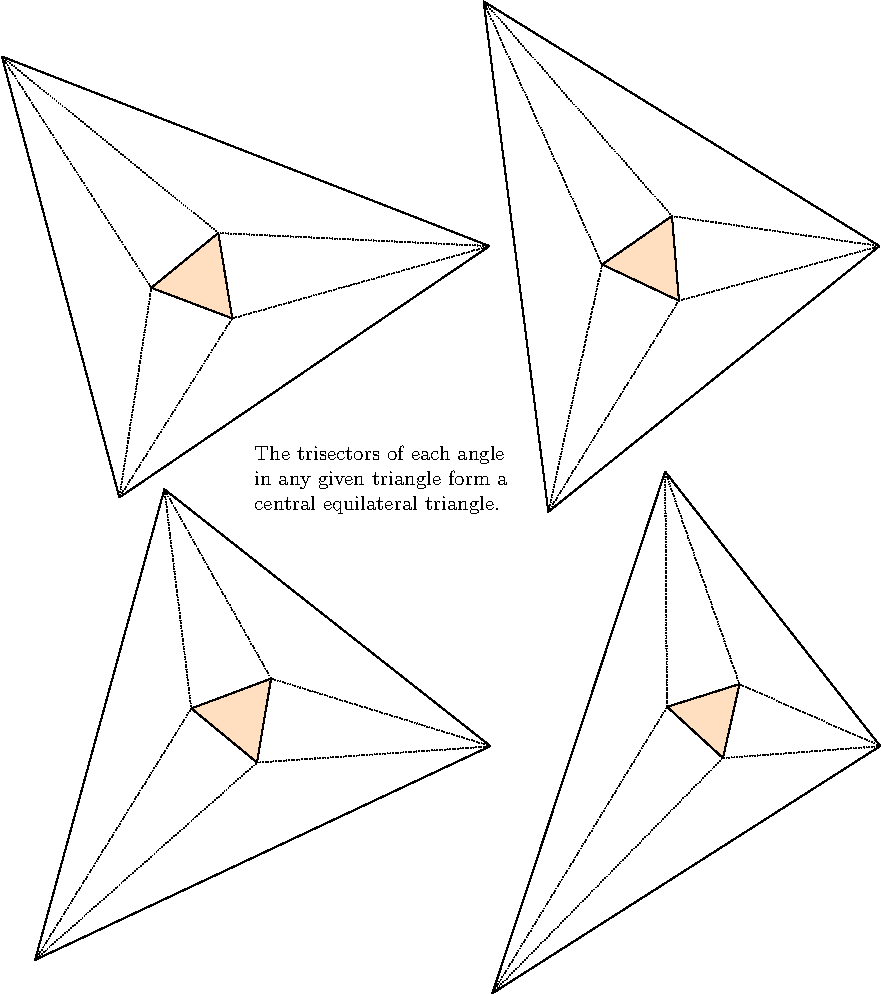
\includegraphics[width=4.2in]{trisection-triangles}\vss}
\vskip-\baselineskip
\begin{code}[xleftmargin=0pt, xrightmargin=-80pt]
randomseed := 2485.81543;
vardef measured_angle(expr p, o, q) = 
   (angle (p-o) - angle (q-o)) mod 360
enddef;
beginfig(1);
picture T;
for i=0 upto 1:
  for j=0 upto 1:
    clearxy;
    T := image(
      z1 = (120 + uniformdeviate 21, 0);
      z2 = (120 + uniformdeviate 21, 0) rotated 120 rotated 21 normaldeviate;
      z3 = (120 + uniformdeviate 21, 0) rotated 240 rotated 21 normaldeviate;
      numeric a, b, c;
      a = measured_angle(z3, z1, z2);
      b = measured_angle(z1, z2, z3);
      c = measured_angle(z2, z3, z1);
      z4 = whatever [z1, z2 rotatedabout(z1, 1/3 a)] 
         = whatever [z2, z3 rotatedabout(z2, 2/3 b)];
      z5 = whatever [z2, z3 rotatedabout(z2, 1/3 b)] 
         = whatever [z3, z1 rotatedabout(z3, 2/3 c)];
      z6 = whatever [z3, z1 rotatedabout(z3, 1/3 c)] 
         = whatever [z1, z2 rotatedabout(z1, 2/3 a)];
      fill z4--z5--z6--cycle withcolor 3/4[red + 1/2 green, white];
      draw z4--z5--z6--cycle;
      draw z1 -- z4 -- z2 -- z5 -- z3 -- z6 -- cycle
           dashed withdots scaled 1/4;
      draw z1 -- z2 -- z3 -- cycle;
    );
    draw T shifted (200i, 240j);
  endfor
endfor
label.rt(btex \vbox{\halign{#\hfil\cr The trisectors of each angle\cr 
in any given triangle form a\cr central equilateral triangle.\cr}} etex, (24, 128));
endfig;
\end{code}
\newpage
\kern-\baselineskip
\vpic{1in}{projections1}

\begin{code}[xleftmargin=0pt, xrightmargin=-72pt]
beginfig(1);
% define the end points of the three rays
z1 = right scaled 200 rotated 10;
z2 = right scaled 100 rotated 135;
z3 = right scaled 225 rotated -17.5;
% define the other points, relative to Q
pair A, B, P, Q, R;
Q = 0.8125 z3;
A = whatever[origin, z1]; A-Q = whatever * z1 rotated 90;
P = whatever[origin, z2]; P-Q = whatever * z2 rotated 90;
B = whatever[origin, z1]; B-P = whatever * z1 rotated 90;
R = whatever[A,Q];        R-P = whatever * (B-P) rotated 90;
% mark the angles
drawoptions(withcolor .67 blue);
draw fullcircle scaled 30 rotated angle (Q-P) shifted P cutafter (P--B);
draw fullcircle scaled 30 rotated angle (P-Q) shifted Q cutafter (Q--R);
draw fullcircle scaled 30 rotated angle P               cutafter (origin--z1);
drawoptions();
% draw the rays and A--Q
drawarrow origin -- z1; label(btex $r_1$ etex, z1 scaled 1.05);
drawarrow origin -- z2; label(btex $r_2$ etex, z2 scaled 1.08);
drawarrow origin -- z3; label(btex $r_3$ etex, z3 scaled 1.05);
draw A--Q;
% draw the dashed lines
draw B--P--R--Q--P dashed evenly;
drawarrow origin -- P scaled 4/3 dashed evenly;
% label the points
dotlabel.urt(btex $Q$ etex, Q);
dotlabel.top(btex $A$ etex, A);
dotlabel.lrt(btex $R$ etex, R) withcolor .67 blue;
label.top (btex $B$ etex, B);
label.llft(btex $P$ etex, P);
label.llft(btex $O$ etex, origin);
endfig;
\end{code}

\newpage
\subsection{Trigonometry functions}\label{trig}

\MP\ provides only two basic trigonometry functions, "sind" and "cosd";  this lack
appears to be a deliberate design.  In general it's much easier to use the "rotated"
and "angle" functions than to work out all the sine, cosines and arc-tangents
involved in rotating parts of your picture.  But if you really want the `missing'
functions they are not hard to implement.

First you might want versions that accept arguments in radians instead of degrees.
For this you need to know the value of $\pi$, but this is not built into plain \MP.
If you are using the default number system then it's enough to define to five
decimal digits,%
\vadjust{\moveright 384pt\vbox to 0pt{\kern-108pt
\begin{code}
numeric pi;
% approximate value
pi := 3.14159; 
% measure round a circular arc...
pi := 1/4 arclength (quartercircle scaled 16);
% up to 34 digits of precision 
pi := 3.141592653589793238462643383279503;
% as many digits as are needed...
vardef getpi =
  numeric lasts, t, s, n, na, d, da;
  lasts=0; s=t=3; n=1; na=0; d=0; da=24;
  forever:
    exitif lasts=s;
    lasts := s;
    n := n+na; na := na+8;
    d := d+da; da := da+32; 
    t := t*n/d;
    s := s+t;
  endfor
  s
enddef;
pi := getpi;

% conversions
vardef degrees(expr theta) = 180 / pi * theta enddef;
vardef radians(expr theta) = pi / 180 * theta enddef;
% trig functions that expect radians
vardef sin(expr theta) = sind(degrees(theta)) enddef;
vardef cos(expr theta) = cosd(degrees(theta)) enddef;
% inverse trig functions
vardef acosd(expr a) = angle (a,1+-+a) enddef;
vardef asind(expr a) = angle (1+-+a,a) enddef;
vardef acos(expr a) = radians(acosd(a)) enddef;
vardef asin(expr a) = radians(asind(a)) enddef;
% tangents
vardef tand(expr theta) = save x,y; (x,y)=dir theta; y/x enddef;
vardef atand(expr a) = angle (1,a) enddef;
\end{code}
\vss}}
but if you are using one of the new number systems you might want more digits of
precision.  In fact there's no harm in always defining these extra digits; even when
you are using the default "scaled" number system, \MP\ will happily read as many
extra digits of $\pi$ as you supply, before it rounds the value to the nearest
multiple of $1\over65536$ (which turns out to be $3.14159$). The same applies to the
"double" and "binary" number systems, but the "decimal" number system will give you
an error if you supply more digits that the default precision (which is 34).  So
it's best to use no more than 34 digits.  It's also possible, but not really worth
the trouble, to define a routine to calculate $\pi$ to the current
precision.  However you define it, once you are armed with a value for $\pi$ you can
then define functions to convert between degrees and radians, and some more `normal'
versions of sine and cosine.

There's no built-in $\arccos$ or $\arcsin$ function but each is very easy to
implement using a combination of the "angle" function and the Pythagorean difference
operator.

\MP\ does have built-in functions for tangents; but they are called "angle" and
"dir" and they are designed for pairs. So $\kw{angle}\,(x,y)=\arctan(y/x)$ while
$\kw{dir}\,30$ gives you the point $(x,y)$ on the unit circle such that $\tan
30^{\circ} = y/x$.  You can use these ideas to define tangent and arctan functions
if you really need them, but often "angle" and "dir" are more directly useful
for drawing.  You should also be aware that the tangent function shown here does not
check whether $x=0$; if this is an issue you can say something like
`$\kw{if}\,x=0\!:\id{infinity}\: \kw{else}\!: y/x \kw{fi}$' at the appropriate
point.


\newpage
\section{Traditional labels and annotations}

\moveright384pt\vbox to 0pt{\hsize 4.2in\vss\textcolor{blue}{\itshape This section describes labels and
annotations in what can be called the traditional \MP\ environment, where your
figures are compiled with "mpost".  The following section describes labels and
annotations in the new-fangled (but rather better) world of "lualatex" and the
"luamplib" package.}\par\kern 16pt}

\noindent
\MP\ does not draw text directly; instead it provides two different mechanisms to
turn a text string into a picture, which can then be treated like any other; in
other words, the text picture can
be saved as a picture variable, drawn directly, or transformed in some way with a
scaling, a reflection, or a rotation.

\subsection{Simple strings in PostScript fonts with \texttt{infont}}

The first mechanism is the primitive binary operation "infont".  As explained in
section~8.3 of the \MP\ manual, it takes two strings as arguments: the left hand
argument is the string of text to be printed; the right hand argument is the name of
the font to use; and the result is a "picture" primary.\vadjust{
\moveright384pt\vbox to 0pt{\kern -126.5 bp
    \hsize 4.2in\noindent
To find the name of a suitable font, you have to consult your local "psfonts.map"
file, and probably the PSNFSS documentation.
Here are a few of the many fonts available on my local \TeX\ installation; the name
to use with "infont" is in the first column.  
$$
\includegraphics{font-sampler2}$$
The text example in the first line
of this table was produced with
\begin{code}
    draw "Grey fox 42" infont "pagk8r" shifted (124,144);
\end{code}
Note that in PostScript terms each of these font names refers to a combination of
three files: an encoding that maps the characters you type to the glyphs in the
font; a font metrics file that defines the sizes of the virtual boxes surrounding
these glyphs; and a set of PostScript routines that actually draw them.  In a \TeX\
installation 
these combinations are defined in a font map file, usually called "psfonts.map".
If you run "mpost" with the "-recorder" switch it will write an extra log file (with
a ".fls" extension) that lists the names of all the files used in a job.
The actual font map file in use will be one of these.  You can then browse it to
find a definitive list of the font names you can use with your local \MP.
\vss}}

To make a suitable string you can enclose your text
in double quotes to make a string token, or to refer to a string variable, or do 
one of these:
\begin{itemize}
    \item Concatenate two other strings with "&".

    \item Use "substr (a,b) of s" to get a substring of string "s".

    \item Use "min(a,b,...)" or "max(a,b,..)" to find the lexicographically smallest
        (or largest) string in the list "a,b,...".  The list must have at least two
        entries, and they must all be strings. 

    \item Use "char" to convert a numeric expression to the corresponding an ASCII
        code;
          the numeric expression is rounded to the nearest integer modulo
          256.
    
    \item Use "decimal" to get
        the value (as a decimal) of a numeric expression.

    \item Apply "str" to any suffix (and hence to any variable).  You get back a
        string representation of the suffix or variable name.

    \item Use "readfrom" to read one line from a file as a string.

    \item Use "fontpart" to extract the name of the font used in a picture created
        with "infont" --- the string will be empty if there's no text element in the
        picture.

    \item Use "textpart" to get the text used in a picture created by "infont" ---
        the string will be empty if there's no text element in the picture.

\end{itemize}

\newpage
\subsubsection{Character sets used by \texttt{infont} to set text} 

Standard \MP\ is configured to accept as input only space and the usual 94 visible
ASCII characters (that is the characters numbered 32 to 126 in the tables at the
right), but you can use any 8-bit characters as the payload of a string. 
However, plain \MP\ is set by default to use "cmr10", the familiar Computer Modern typeface
developed by Knuth for \TeX, and unfortunately, this is encoded using the \TeX\ text
font encoding (also known as `OT1', and as shown in the first table in Appendix~F of the {\sl \TeX book}).  
\mpic{-72pt}{font-sampler1.pdf}  
From the point of
view of using "infont" to make simple labels, this means that the characters for
space and seven other characters ("< > \ _ { | }") are in the wrong place.  
You are likely to notice this first if you try to set a label with two words; the
space will come out as a small diagonal stroke accent that is used in plain \TeX\
to make the characters Ł and ł, used in Polish and other Slavic languages.

To fix this you should change the default font at the start of your program:
\begin{code}
defaultfont := "texnansi-lmr10";  % for Computer Modern Roman
\end{code}
If you want "cmss10", use "texnansi-lmss10" and so on.  The encoding is shown on the
right.  The characters printed in black correspond to the widely used ISO Latin~1
encoding.  If you want to use one of the standard PostScript fonts listed on the
previous page, then the encoding to use is "8r".  As you can see from the lower
table, this is nearly the
same; for most users the main difference is the location of the Euro currency
symbol.
   
Choosing a font with one of these encodings means that if you use Windows code page
1252 or ISO Latin 1 as the encoding for your text editor, you can create labels with
accented characters using "infont" and without resorting to "btex" \dots\ "etex".
But if you are using UTF-8 characters (as many of us are now), then you have to do
some extra work to get them printed correctly with "infont".  A solution is shown on
the next page.  

In the normal course of labelling a drawing, it is always possible to
use "btex" \dots\ "etex" to produce your accented characters as discussed in section
\ref{btex} below; but it may be that you are using \MP\ to represent data and labels
supplied from some other program or a website.  In this case it can be useful to be
able to work with at least a subset of UTF-8 input.

\newpage
\subsubsection{Mapping a subset of UTF-8 for \texttt{infont}}

UTF-8 is a way of
representing 16-bit Unicode characters with sequences of 8-bit characters. So your
UTF-8 aware editor may show you an é but \MP, knowing nothing about UTF-8,
will see this as é.  But you can write a fairly simple routine to decode the
commonly used subset of
UTF-8.\vadjust{\moveright5.5in\vbox to 0pt{\hsize4in\vskip -9.5pt\parindent 0pt
\def\item{\leavevmode\llap{•~}}
\item You can extend this idea to cope with other UTF-8 characters, including 
  those that use three bytes.  The UTF-8 page on Wikipedia shows you how it
  works.  Essentially you look at the values of the next 2 or 3 characters and
  then pick the appropriate character in your encoding with "char".  But your
  output is still, of course, limited to the 256 characters in your font.

\item If you get tired of writing "decode", you could define a short cut with a
  shorter name.  You could even write it as a primary without parentheses like
  this:
\begin{code}
def U primary s = if string s: decode(s) fi enddef;
\end{code}
which would let you write:
\begin{code}
label.rt(U"café à la möde", (x,y));
\end{code}

\item However, there's no point in making any of this too elaborate.  If you
  really want proper Unicode support you should use \MP\ with Lua\TeX.
\vss}}
\begin{code}[xrightmargin=-10pt]
vardef decode(expr given) = 
  save a,i,s,out; string s, out; numeric a, i;
  out = ""; i=0;
  forever:
    i := i+1; s := substring (i-1,i) of given; a := ASCII s;
    if a < 128: 
    elseif a = 194: 
      i := i+1; s := substring (i-1,i) of given;
    elseif a = 195: 
      i := i+1; s := char (64 + ASCII substring (i-1,i) of given);
    else: 
      s := "?";
    fi
    out := out & s;
    exitif i >= length given;
  endfor
  out
enddef;
\end{code}
Use it with "infont" like this: \verb|decode("café") infont "ptmr8r"| to produce a
normal "picture" that can be passed to "draw" or saved as
usual.\vadjust{\moveright5.5in\vbox to 0pt{\hsize4in\vskip -9.5pt
\noindent The fragment on the left produces:
$$
\includegraphics{utf82}$$
The \texttt{label} macro automatically calls \texttt{infont} with the current value
of \texttt{defaultfont}; notice how it also adds some extra space.
\vss}} 
\begin{code}
draw "café noir £2.50" infont "pncr8r";
draw decode("café noir £2.50") infont "pncr8r" shifted 12 down;
defaultfont := "pncr8r";
label.rt("café noir £2.50", 24 down);
label.rt(decode("café noir £2.50"), 36 down);
\end{code}
Note that you can't just use "draw" with a string variable; you have to use
"infont" to turn the string into a picture.
On the other hand, "label" calls "infont" automatically, but you must explicitly set
the default font, preferably to one with an encoding that 
is compatible with ISO Latin~1.


\newpage
\subsubsection{Typographical minus signs with \texttt{infont}}

If you are producing labels for a numeric reference scale, like the axis of a chart,
it is convenient to be able to write a loop like this (assuming "u" is a horizontal
unit):
\begin{code}
for x=1 upto 10: label(decimal x, (x*u,-5)); endfor
\end{code}
to produce your labels, however if "x" is negative this does not come out so well,
because the first character of the string produced by "decimal -1" is an ASCII 45,
which is the hyphen character.  What we need is the mathematical minus sign instead;
this is what you get with "btex $-1$ etex" of course, but that's hard to put in a
loop.  Instead you can do this:\vadjust{\moveright5.5in\vbox to 0pt{\vss\hsize4in
$$
\includegraphics{minus1}$$
\vss}} 
\begin{code}
string minus_sign;
minus_sign := char 143; % if you are using the texnansi encoding
minus_sign := char 12;  % if you are using the 8r encoding
for x=-10 upto 10: 
   label(if x<0: minus_sign & fi decimal abs(x), (x*u,-5)); 
endfor
\end{code}
Note that this does not work with the default encoding used in "cmr10" because
there is no minus sign available in that font.  Plain TeX uses "char 0" from
"cmsy10".

\subsubsection{Bounding boxes and clipping with \texttt{infont}}

Once the encoding is fixed, the other two parts of a PostScript font are the font
metrics and the programs that draw the actual glyphs.  The font metrics define the
width of each character and provide a kerning table to adjust the space between
particular pairs.\vadjust{\moveright5.5in\vbox to 0pt{\vss\hsize4in
$$\includegraphics{infont-example1} \qquad \includegraphics{infont-example2} $$
}} This means that certain characters will overlap each other or stick out
beyond the bounding box of the picture produced by "infont".  This is not normally a
problem unless the picture happens to be at the edge of your figure.  In the first
example observe how the first and last letters have been clipped; in the second a
wider baseline has been added to prevent this.  
If you want this effect, but you
don't want to see the baseline, then draw it 
using the colour "background".

\subsubsection{But what about the \texttt{label} command?}

As a convenience, the plain \MP\ format provides a "label" macro that automatically
turns strings into pictures for you using whatever font name is the current value of
"defaultfont" and scaled to the current value of "defaultscale".\vadjust{\moveright5.5in\vbox to 0pt{\vss\hsize4in
\noindent
The "label" macro is defined (essentially) to do this:
\begin{code}
    def *label(expr s, z) = 
      draw s if string s: infont defaulfont 
                          scaled defaultscale fi shifted z
    enddef;
\end{code}
plus some slightly-too-clever code to align the label for you.
}}

\newpage
\subsubsection{Bounding boxes and alignment with \texttt{infont}}
\label{infontbbox}

To allow you to align a text label on a specific point, \MP\ provides five unary
operators to measure the bounding box of a picture; they are shown in
\textcolor{red!67!black}{red} in the diagram, and you can use them to measure the
width, depth, and height of a textual picture.  You can also work out the location
of the baseline of the text or the x-height, provided you know how much your picture
has been shifted.
The easiest way to do this is to 
measure the picture \textit{before} you shift it.\vadjust{\moveright5.5in\vbox to 0pt{\vss\hsize4in
$$\includegraphics{infont-example3}  $$
\vss}}
\begin{code}
    picture pp; pp = "proof" infont "pplri8r";
\end{code}
Here the picture \id{pp}
is created with the origin of the text sitting at coordinates $(0,0)$;
then you can get the dimensions like this
\begin{code}
    wd = xpart urcorner pp;
    ht = ypart urcorner pp;
    dp = ypart lrcorner pp;
\end{code}
In this particular case you will find that you have $wd=20.47292$, $ht=7.19798$, and 
$dp=-2.60017$.  The depth is negative because the descenders on the
\textdemo{\textit{p}} and the \textdemo{\textit{f}}
in the chosen font stick down below the base line.  The height is greater than the
x-height, because the \textdemo{\textit{f}} also sticks up, so you need to make another measurement:
\begin{code}
numeric xheight; xheight = ypart urcorner ("x" infont "pplri8r");
\end{code}
Armed with these measurements you can align your text labels neatly so that they are
all positioned on the base line or vertically centered on the lower case letters
regardless of any ascenders or descenders.  To draw your label left-aligned with its
origin at position $(x,y)$ you just need to use: \kw{draw} \id{pp} \kw{shifted} $(x,y)$.  
To draw it right-aligned, you subtract
\id{wd} from the $x$-coordinate: \kw{draw} \id{pp} \kw{shifted} $(x-wd,y)$.  Or to
centre it, subtract $1/2wd$.  To center it vertically on the lowercase letters,
subtract $1/2\id{xheight}$ from the $y$-coordinate.  You might of course like to
wrap these adjustments up in your own convenient macro to help you maintain
consistency in a diagram with many labels.

Alternatively you can adjust the bounding box of your textual picture and then use
it with "label" as normal.  Assuming \id{wd} is set to the width of your picture
and \id{xheight} is set correctly for the current font, then 
\begin{code}
    setbounds pp to unitsquare xscaled wd yscaled xheight;
\end{code}
will make the "label" alignment routines ignore any ascenders or descenders.  
%Beware
%that if the resulting label is right at the edge of your drawing then any parts of
%the text that stick out of the adjusted bounding box will be clipped.

\newpage
\subsubsection{Setting greek letters with \texttt{infont}}

\leavevmode\hbox{}
$$\includegraphics[width=0.5\textwidth]{greek-homer.pdf}$$
While it's technically possible to set the whole of Homer's \textsl{Iliad} using the Greek
fonts available to \MP, it's probably not a great use of time; on the other hand you
might want to label parts of a diagram with Greek letters, and for single Greek
letters "infont" is more than adequate.

The Greek letters for Computer Modern are in the maths-italic font "cmmi10", which
uses the encoding shown on p.\thinspace 430 of \textsl{The \TeX{}book}.  For historical
reasons there's no omicron available, so you are supposed to use the $o$~character
instead.  Fortunately you are unlikely to need more than the first few, and it's
quite easy to remember that $"char 11"=\alpha$, $"char 12"=\beta$, and so on.
Producing the upper case letters is a bit more of a fiddle with this encoding as you
need to know which ones use a Roman letter form; for details examine the program on
the right, or check the table on p.\thinspace\pageref{eulertable}.
Herman Zapf's elegant Euler font, available as "eurm10" uses the same encoding and
makes a refreshing change for some diagrams.\vadjust{\moveright5.5in\vbox to
0pt{\hsize4in\kern-164pt
\begin{code}
beginfig(1);
string ab, AB;
ab = ("" for i=11 upto 23: & char i endfor 
   & "o" for i=24 upto 33: & char i endfor);
AB = ("AB" & char 0 & char 1 & "EZH" & char 2 & "IK" 
          & char 3 & "MNO" & char 4 & char 5 & "P"
          & char 6 & "T"   & char 7 & char 8 & "X"
          & char 9 & char 10);

draw ab infont "cmmi10";
draw AB infont "cmmi10" shifted 12 down;
draw ab infont "eurm10" shifted 32 down;
draw AB infont "eurm10" shifted 44 down;
endfig;
\end{code}
\centerline{\includegraphics{greek1}}

\begin{code}
string ab, AB;
ab = "abgdezhjiklmnoxprstufqyw";
AB = "ABGDEZHJIKLMNOXPRSTUFQYW";
\end{code}
\centerline{\includegraphics{greek2}}
\vss}}

\medskip\noindent
If you have fonts installed from the Greek Font Society, then you get a wider
choice, and a slightly more modern encoding.  All of the letters are available in the
normal ASCII positions, so you do not have to muck about with "char xx".  

\vbox to 0pt{\centerline{\includegraphics{gfs-encoding.pdf}}\vss}



\newpage
\subsection{Setting text with \texttt{btex} and \texttt{etex}}\label{btex}

As soon as you need anything complicated in a label, like multiple fonts, multiple
lines, or mathematics, you will find it easier to switch from "infont" to the
"btex ... etex" mechanism that calls \TeX\ to create your textual picture.  In fact
you might prefer to use \TeX\ for all your labels, even simple strings, for the sake
of consistency.  The only downside is that this mechanism is a little bit slower.

The "btex" mechanism produces a textual picture just as "infont" does with a height,
width, and depth that you can measure, and adjust, as discussed in
section~\ref{infontbbox}.  And again, just like "infont" you can either use "draw"
to place the resulting picture directly, or pass it to the "label" macro.

What you need to be aware of is that \MP\ places everything you put between the "btex" and
"etex" into an "\hbox{...}" and processes it with plain \TeX.  This has several
implications, especially if you need to make your diagrams match the formatting of a
particular \LaTeX\ format.

\subsubsection{Matching the fonts with plain \TeX}

Despite the apparent restriction of using plain \TeX\ it is almost always possible
to match the font and format of an enclosing \LaTeX\ document. 
The simplest approach is to use the plain
\TeX\ font mechanism with the names from "psfonts.map".  
\begin{code}
verbatimtex
\font\rm=ptmr8r\rm
etex
\end{code}
Adding this at the top of your \MP\ program will set your text in Times New Roman,
although any maths will still be set using Computer Modern.  
To fix this, all you
have to do is to redefine all the maths fonts in all sizes you need; this is not really
that hard but it is a fiddle to get all the details right.  Fortunately
the wonderful "font-change" package has done it all for you for a large range of
fonts; with this package installed you can use
\begin{code}
verbatimtex
\input font_times
etex
\end{code}
instead, and all of your \TeX\ labels, including bold letters, italics, small caps,
and mathematics will be set in Times New Roman.\vadjust{\moveright5.5in\vbox to
0pt{\hsize 4in\vss\noindent
Here are some samples of the fonts available in the "font-change" package.  For full
details, and especially details about using AMS symbols, see the package
documentation.
$$\includegraphics{font-sampler3}$$
}}

\newpage
\subsubsection{Matching fonts using \LaTeX}
If you still can't get your labels to match, you can force \MP\ to use \LaTeX\
instead of plain \TeX\.  You need to use the "-tex" command line switch:
\begin{code}
    mpost -tex=latex
\end{code}
and also load whatever packages you need in a "verbatimtex" block at the top of your
\MP\ file.
\begin{code}
verbatimtex
\documentclass{article}
\usepackage{mathpazo}
\usepackage{xcolor}
\begin{document}
etex
\end{code}
Note that the "\documentclass" and the "\begin{document}" lines are required, but
\MP\ is smart enough to add an "\end{document}" for you.

\MP\ needs a ".dvi" file to work with, so you can only use "latex" or "elatex", and
not any of the more modern engines, like "pdflatex".  Generating the labels takes a
little bit longer because you have to load rather more `infrastructure' for \LaTeX,
and you are limited to whatever font packages you have that work with the
traditional \LaTeX\ engine. 

\subsubsection{Getting full access to your system fonts}

If you want full access to all of your system fonts you can
approach the problem the other way round and use one of the various means to include
\MP\ graphics as part of your \LaTeX\ source code.  These include "gmp" for
pdf\LaTeX, "luamplib" for lua\LaTeX, and the whole Context system.  The great
advantage of these systems is that all of your \MP\ labels directly inherit the
environment of the parent document, and give you access to all your system fonts and
full Unicode support -- the only disadvantages are that it's not so fast or simple as plain \MP\
and you have to compile every graphic everytime you compile the document.  It is of course always possible to
use these systems to produce standalone PDF graphics that you can then include in a
more conventional \TeX\ document.  The example on the right shows how;  in this case
the text uses the fonts set in the \LaTeX\ preamble.\vadjust{\moveright5.5in\vbox to
0pt{\hsize 4in\vss\noindent
Here is a version of the Lua logo, with a Unicode accent for show.
$$\includegraphics[scale=0.7]{lulu.pdf}$$
produced with "luamplib":
\begin{smallcode}
\documentclass[margin=5mm]{standalone}
\usepackage{fontspec}
\setmainfont{TeX Gyre Heros}
\usepackage{luamplib}
\begin{document}
\begin{mplibcode}
beginfig(1);
color lemon, midnight; lemon = (1,1,1/2); midnight = (0,0,1/2);

fill unitsquare shifted -(1/2,1/2) scaled 4cm withcolor lemon;
fill fullcircle scaled 3cm withcolor midnight;
draw fullcircle scaled 3.7cm dashed evenly scaled 2 withcolor .5 white;

fill fullcircle scaled 8mm shifted (0.7cm,0.7cm) withcolor white;
fill fullcircle scaled 8mm shifted (1.4cm,1.4cm) withcolor midnight;

label.bot(btex Luã etex scaled 2.8,origin) withcolor white;
endfig;
\end{mplibcode}
\end{document}
\end{smallcode}
}}

% new page
\subsubsection{Producing display maths}

As noted above, \MP\ places everything you put between "btex" and "etex" into an
"hbox" and typesets it in restricted horizontal mode.  One of the restrictions in
this mode is that you can't use "$$ ... $$" to produce display maths. This means that  
the various mode-sensitive constructs like $\sum$ and $\int$ will come out in their
smaller forms.  If you want them big, then the solution is simple: just add
"\displaystyle" at the beginning of your formula.\vadjust{\moveright5.5in\vbox to 0pt{\hsize 4in\vss\noindent
\begin{code}
...
label(btex $\displaystyle \int_0_t 3x^2\, dx$ etex, (x,y));
...
\end{code}
}}

\subsubsection{Multiline text labels}

Another consequence of the "hbox" feature is that there is no automatic text
wrapping done for you, but again you can work round this easily because \TeX\ lets
you nest a "\vbox" inside an "\hbox".  This gives you proper paragraph-like wrapping
but you will almost certainly need to adjust the line length, justification, and paragraph
indentation.\vadjust{\moveright5.5in\vbox to 0pt{\hsize 4in\vss\noindent
\begin{code}
...
label(btex \vbox{\hsize 2in\parindent 0pt\raggedright
    An extended caption or label that will be set as a 
    small paragraph with automatic hyphenation and line-wrapping.
} etex, (x,y));
...
\end{code}
}}

You will only need the full power of \TeX's paragraph making system occasionally
though: more usually you will just have one or two lines in each label, and you
might be quite happy to control the line breaks manually.  In this case it's helpful
to wrap a little tabular structure around your text.  Here's how to define something
suitable in plain \TeX.  First you need to define a suitable macro at the start of
your figure
\begin{code}
verbatimtex
\def\s#1{\let\\\cr\vbox{\halign{\hfil\strut ##\hfil\cr#1\crcr}}}
etex
\end{code}
then you can write labels like this:
\begin{code}
...
label(btex \s{Single line} etex, z1);
label(btex \s{Longer text split\\onto a new line} etex, z2);
...
\end{code}
Notice how you can still use the macro with single lines, you just get a one-line
table as it were. 
Note also that the definition of "\s" as given will centre each line of the text under
the one above.  If you want them left aligned or right aligned, omit one of the
"\hfil" commands.

You can of course achieve the same effects using \LaTeX\ tabular structures, but
then you have to use the "-tex=latex" option to run
\MP.\vadjust{\moveright5.5in\vbox to 0pt{\vss\hsize4in\noindent
        \textbf{Note}: In case it's not obvious, if you want text wrapping or
        tabular arrangements as discussed here, you need to use \texttt{btex ... etex}
        to set your labels.  There's no text wrapping with "infont".  On the other
        hand if all of your labels are in "infont" but you just want one extra that
        has two lines, you can split the text into two separate labels and position
them independently.}}

\subsubsection{Dynamic labels}

If you are a maven of programming language syntax you may have noticed that 
"btex ... etex" fits into the type system that \MP\ inherits from \MF\ as a "picture" and
not as a "string".  Effectively "btex" and "etex" act as a special pair of quotation
marks that create a picture; however the contents are used verbatim, so that the
whole contruction is a syntactical atom.  This means that you \textbf{cannot} write
this sort of thing: 
\begin{code} 
for i=0 upto 4: % this won't work
  label(btex "$p_" & decimal i & "$" etex, (10i,0)); 
endfor 
\end{code} 
Given this input \MP\ would attempt to get \TeX\
to typeset 
\begin{code}
\hbox{"$p_" & decimal i & "$"}
\end{code}
which would probably result in a
`Misplaced alignment tab character' error.
To get round this problem, \MP\ provides a general mechanism to write out a
string to a file, and then read the file back in.  This is the mechanism used by the
"TEX()" macro that is provided alongside "plain.mp".  This allows you to write:
\begin{code}
input TEX
...
for i=0 upto 4:
  label(TEX("$p_" & decimal i & "$"), (10i,0));
endfor
\end{code}
This works because the TEX macro is expecting a "string" so the normal string
concatenation rules are applied.  The macro wraps the result with "btex" and "etex",
writes them out to a file, and then reads the file in again so that \MP\ gets the
correct contents to pass to \TeX.  

The only trouble with this is that it makes \MP\ open a file,
write to it, close it, and then read it in again for each label one at a time; this
means that it's very slow.  
The example on the right shows how to speed things up, by using the same file for
all the labels and only writing it once.
The "write" command is a \MP\ primitive, and "EOF" is defined in "plain.mp".%
\vadjust{\moveright5.5in\vbox to 0pt{\vss\hsize4in\noindent
\begin{code}
path c; c = fullcircle scaled 100; draw c withcolor .67 red;
for i=0 upto 7:
  fill fullcircle scaled 3 shifted point i of c;
  z[i] = point i of c scaled 1.15;
  write "label(btex $p_" & decimal i & "$ etex,(" 
        & decimal x[i] & "," & decimal y[i]
        & "));" to ".mplabels";
endfor
write EOF to ".mplabels";
input ".mplabels";
\end{code}
$$
\includegraphics{dynamic-labels2}
$$
Note that you can't use "decimal" on a "pair" variable, but you can save the pair
as a "z"-variable and then use the "x" and "y" syntax.  The scaling trick used here
only works because "c" is centered on the origin.  If "c" were drawn elsewhere, you
would have to write:
\begin{code}
... point i of c shifted -center c 
                 scaled 1.15 
                 shifted center c ...
\end{code}
}}

\newpage
\subsection{Markers for annotations}

\subsubsection{Call outs}


- annotations - overbrace, underbrace, length arrows etc, ahangle trick

\newpage
\section{Modern labels and annotations}

This section is a re-working of the previous section, that attempts to show how much
nicer it is to handle labels in the new world of `luamplib`.


\newpage
\section{Line caps and line joins}

The PostScript language defines parameters that affect how the ends of each line are
drawn and how lines are joined together.  Plain \MP\ provides access to these
parameters through internal variables called "linecap" and "linejoin"; it sets both
of them to the value "rounded" at the start of each job. 
\mpic{0pt}{basic_drawing1}





The figure on the right shows the affect of the different settings, using an
exaggerated line width of 2 points (instead of the usual 0.5 points).  Some
observations
to note:
\begin{itemize}
    \item When $\id{linecap}=\id{squared}$ then \kw{drawdot} produces diamond-shaped
        dots, even when you are drawing with the default circular pen. 

    \item When $\id{linecap}=\id{butt}$ then \kw{drawdot} produces invisible dots.
        They still count towards the bounding box of the picture but there's no mark
        on the page.

    \item When $\id{linecap}=\id{squared}$ then \kw{drawarrow} produces some
        unpleasant results; even when $\id{linejoin}=\id{mitered}$, you can still
        see small jaggies on the slopes of the arrows.

    \item The arrows are nice and sharp when 
        $\id{linejoin}=\id{mitered}$, but they over shoot the mark slightly.

    \item If you zoom in, you can see the effect of $\id{linejoin}$ on the corners of the grey box
        as well as on the arrow heads, but you might not notice the difference when
        the picture is printed unless you have a very high resolution printer.

    \item 
        This drawing was done with \mpl{pencircle scaled 2}, so that the dots 
        would be easy to see. This does make the arrows drawn with the 
        default line modes (rounded caps and rounded joins) looks a bit fat;
        they look better with the usual \mpl{pencircle scaled .5}.

\end{itemize}

There is one more PostScript parameter affecting line joins. \MP\ makes it available as "miterlimit" 
and it affects how much a mitered join is allowed to stick out at each corner.  Plain \MP\ sets
"miterlimit=10;" which is correct for nearly all drawings.  If you set
"miterlimit:=0;" then the mitered line join mode becomes more or less the same as the
beveled mode.

\newpage 
\section{Cycloid and other spiral graphs}

This section examines cycloids; the curves made by points on the circumference of a
rolling wheel.  In the first diagram the cycloid is drawn in red and the
corresponding rolling wheel in blue.  The main idea in this diagram is to make the
whole drawing depend on just a few parameters;  here there are two: the radius $r$
and the amount of rotation $θ$.  If we make $r$ bigger, the drawing will be
scaled up; if we change $θ$, the wheel will appear to have rolled along.
\mpic{-66pt}{cycloids1}


\marginpar{\par\kern1in
\begin{itemize}
    \item Near the beginning we define $\pi=3.14159265$, as there’s no such constant
        built in, but it makes the source more understandable to write "pi/180"
        instead of "0.017453".  It would be nice to use the Greek letters themselves
        in the source, but \MP\ only lets you use plain ASCII characters, to you
        have to write "pi" instead.  Later on "t" is used instead of $\theta$.

    \item The cycloid path "c" is defined using an inline "for" loop.  There’s a
        slight awkwardness to doing this as you have to repeat yourself either at
        the beginning or the end, because you can’t have a dangling "--" or ".." at
        the end of the path.  With a cyclic path it’s easier because you can just
        put "--cycle" after the "endfor".  The strange numbers here are because
        we are going from a rotation of $-100°$ to $+460°$; $360°$ corresponds to
        one hop of the cycloid. 

    \item The axes are done in the usual way, except that we use "xpart" and the
        "point .. of .." notation to make the $x$-axis neatly line up with the ends
        of the cycloid path.

    \item To label points with dots but no text it’s convenient just to fill a
        circle scaled to "dotlabeldiam"; this internal parameter is the current size
        to be used for the dots in "dotlabel".  
    
\end{itemize}}

\mpexternal[xleftmargin=0pt]{cycloids.mp}

\noindent
You can generalize the picture to make cycloids where the point tracing the
cycloid is not on the circumference doing the rolling; the classic example is the
wheel of the train with a flange.  Here I have added $R$ to define the radius of an
outer rim, while the wheel still rolls along a circle of radius $r$.
\mpic{-40pt}{cycloids-extra1}
You might like to experiment with making $R<r$. Note also that variable names are
case sensitive in \MP.

\mpexternal[xleftmargin=0pt]{cycloids-extra.mp}

\noindent The output\mpic{-122pt}{cycloids-extra1} is repeated at the right to save you flicking pages.


\newpage
\section{To do...}


filling shapes
gradients
- faking transparency, overlaying colours, clipping to shapes, filling with patterns
- making waves

- paths, points, directions, subpaths, reversed paths

- boxen, fitting, corners and centres, cutbefore cutafter

- inline if and for and range, loops exitif upto downto

- dots, dotlabeldiam, coloured dots, hollow dots


- graphs, axes, grids, number labels, jitter, sketch graphs


- geometry - constructions, perpendiculars, bisection, tangents, segments and lines,
  incircle, circumcircle, inversion

- angle marks, including curved angle marks

- intersections, buildcycle, eggs, ellipses


- drawing knots, double lines, ropes


- HSV colours, brewer colours, rainbows, 50\% white etc

- decorating lines, Meccano


- finding supremum

- decorated tables

- numberlines


- a pulse

- reuleaux polygons

- the eye

- feynman diagrams the easy way

- physics diagrams, light rays, pendulum, indicating movement and vibration

- parametric equations, folium of Descartes

- examining a glyph

- tesellations and tiling (reference title page)

- all sorts of arrow, arrows between arrows, arrows next to a path (handles)

- faking 3d


- recursive drawings, trees

- four box model charts - Tufte charts - venn diagrams

- my workflow 
- tex process flow diagrams

- triangle of polygons

\newpage
\section{A tour of the plain format}
\newpage
\tableofcontents
\end{document}
